\documentclass{article}
\usepackage{graphicx}
\usepackage[affil-it]{authblk}
\usepackage{url}
\usepackage{nth}
\usepackage{float}
\usepackage{multirow}
\usepackage{hyperref}
\usepackage{subfig}
\usepackage{amsmath}
\usepackage{csquotes}
\usepackage{listings}
\usepackage{tikz}
\usepackage{enumitem}
\usepackage{tabularx}
\usepackage{ltablex}

\usetikzlibrary{matrix}
\usetikzlibrary{decorations.text, decorations.pathreplacing}
\usetikzlibrary{calc}
\usetikzlibrary{arrows.meta}
\usetikzlibrary{intersections}
\usetikzlibrary{positioning}

\renewcommand{\subsectionautorefname}{section}
\renewcommand{\subsubsectionautorefname}{section}

\begin{document}

\title{Developing a driver for a film scanner by means of USB sniffing and reverse engineering}
\author{Hugo Platzer \\ University of Salzburg, Austria}
\maketitle

\begin{abstract}
An open-source driver for a film scanner (Reflecta CrystalScan 7200) is created using
reverse engineering techniques. The USB communication between the device and
the supplied vendor software is recorded and analyzed. As a first stage, the transferred
image is reconstructed from the recording.  After that, a program that closely models
that communication is created to perform scanning without the vendor software.
Patterns in the transferred data are studied so scan parameters can be customized.
Image processing operations relevant to optimizing scanner images are described.
The final driver allows for basic operation (receiving usable images) of the device.

\end{abstract}

\section{Introduction}

For many vendors of consumer electronic devices,
developing drivers for desktop operating systems
with a small market share (such as Linux distributions) is not a priority. Even if
they do develop them, their software usually remains closed-source, which can be considered
undesirable from a security and maintainability standpoint. And even for those
vendors releasing open-source drivers, the device's communication protocol generally remains
undocumented.

This paper focuses on a scanner for film material. The communication between the
device and the supplied Windows software is recorded and analyzed. Based on this analysis,
a working driver supporting basic scanning functionality is created.
It allows the scanner to be controlled without the vendor-supplied software,
making it directly usable under Linux. Also, the device-driver communication
becomes more transparent to developers.

\subsection{The test device}

The Reflecta CrystalScan 7200 is a device for digitizing 35mm film material like
slide, color negative and black-and-white negative film.
It uses a linear CCD sensor on a head moving vertically to record the image on a row-by-row basis.
The maximum scan resolution is 7200 dots per inch which amounts to around 70 megapixels
on a 35mm film frame. It also has a feature called Digital Image Correction and Enhancement:
In addition to red, green and blue, it also records an infrared image of the film.
The dyes in color film are transparent to infrared light,
but dust is not, so the information from this channel is useful for removing it in software.
This scanner is connected via USB \cite{rcs} \cite{rcs_review}.

\begin{figure}[H]
  \caption{Reflecta CrystalScan 7200}
  \centering
  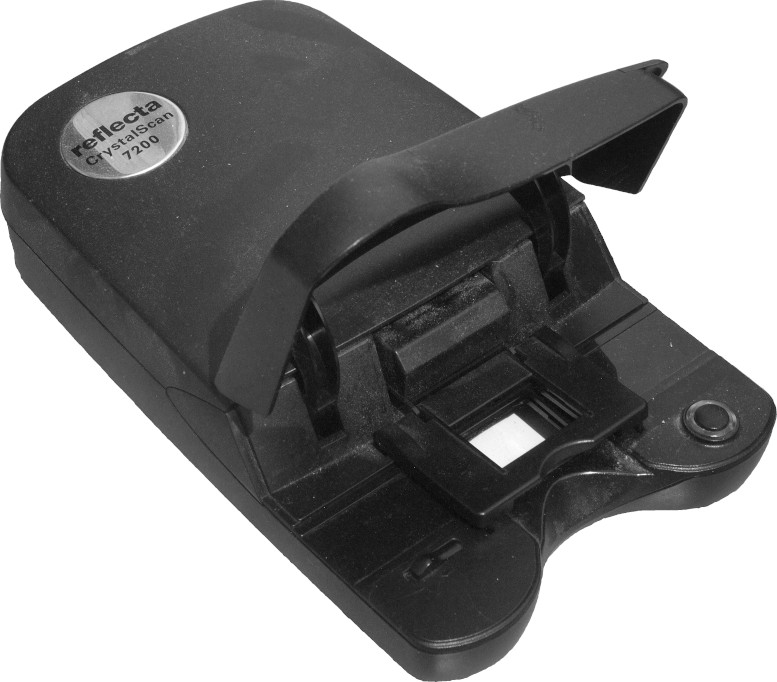
\includegraphics[width=0.5\textwidth]{images/jpg/device.jpg}
\end{figure}

\subsection{Software support}

Reflecta supplies a software called CyberView X5 with the scanner that
provides basic functionality (adjust resolution, scan area, image processing parameters, dust correction).
The software only runs on the Windows and macOS operating systems.

For the Linux operating system, there is a community effort to build scanning software
called SANE (Scanner Access Now Easy) \cite{saneproject}. As opposed to vendor-supplied software, it supports many scanners
from various manufacturers. Unfortunately, the test device was not yet supported.
There exist third-party software products that support this scanner: VueScan \cite{vuescan}
and SilverFast \cite{silverfast}. VueScan also runs on Linux. These, however, are commercial software
and not open-sourced.

\subsection{Reverse engineering}

Since there is no publicly available documentation on how a driver should control this
device, reverse engineering was attempted.
Reverse engineering is the process of reconstructing a specification from a finished
product. Typically, the finished product is software or some sort of electronic
appliance.
Using only resources available to the end user (like hardware,
software / firmware in machine code form, communication channels)
one tries to gain understanding about the inner mechanisms of the product.

In my case, I recorded and analyzed the activity on the USB bus while the scanner
was communicating with the vendor-supplied software.

\section{The USB standard}
\label{sec:usb}

USB (Universal Serial Bus) is an interface intended to connect various peripherals to PCs. These include:
human interface devices like keyboards and mice; storage devices like card readers,
external hard disks, memory sticks and smartphones; multimedia devices like microphones, speakers,
cameras and scanners. Some highlights leading to its wide adoption \cite[p. 11]{usbstd} are:

\begin{itemize}
  \item Unified interface for all kinds of peripherals
  \item Plug and play: the user plugs in the device, the configuration (e.g., loading the appropriate drivers)
  is done automatically by the operating system
  \item Number of ports can be increased using hubs. Multiple hubs can be chained
        allowing for up to 127 devices on a single root port.
  \item High data rate of 480 Mbit / s (USB 2.0 high-speed mode). Also offers low-latency
        transfers for real-time audio/video applications
  \item Backwards compatibility: Older USB 1.1 devices can be used at 2.0 hosts.
        High-speed USB 2.0 devices can also be used on older
        machines supporting only USB 1.1 (albeit at lower speed).
\end{itemize}

\subsection{Electrical side}

A USB cable has four wires: one as ground, VBUS for a 5 V power supply and two for data transmission (\autoref{fig:usbcable}).
The power line allows it to draw up to 100 mA without any configuration. This is useful for simple
devices that are not using the data lanes, just the power, like USB lights. Also it allows for devices
not taking much power to be self-powered which eliminates the need for an extra power supply and connector.
Devices can ask the host for more power (up to 500 mA), those that need even more (like a lot of scanners) need
an external supply \cite[p. 17f.]{usbstd}.

\begin{figure}[H]
  \caption{USB cable cross-section (after \cite[p. 17]{usbstd})}
  \centering
  \scalebox{2}{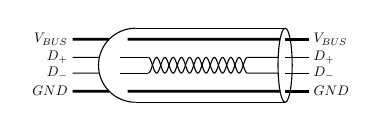
\begin{tikzpicture}
\usetikzlibrary{intersections}

\path[draw,name path=ellipse] (0, 0) ellipse (0.09 and 0.47);
\draw (0, 0.47) -- (-1.90, 0.47);
\draw (0, -0.47) -- (-1.90, -0.47);
\path[draw,name path=circle] (-1.90, 0.47) arc (90:270:0.47);

\node[anchor=west,scale=0.5] at (0.3, 0.33) {$V_{BUS}$};
\node[anchor=west,scale=0.5] at (0.3, 0.1) {$D_+$};
\node[anchor=west,scale=0.5] at (0.3, -0.1) {$D_-$};
\node[anchor=west,scale=0.5] at (0.3, -0.33) {$GND$};

\draw[line width=1] (0.3, 0.33) -- (0, 0.33);
\draw (0.3, 0.1) -- (0, 0.1);
\draw (0.3, -0.1) -- (0, -0.1);
\draw[line width=1] (0.3, -0.33) -- (0, -0.33);

\path[name path=line1] (-2.7, 0.33) -- (0, 0.33);
\path[name path=line2] (-2.7, 0.1) -- (0, 0.1);
\path[name path=line3] (-2.7, -0.1) -- (0, -0.1);
\path[name path=line4] (-2.7, -0.33) -- (0, -0.33);

\path [name intersections={of=ellipse and line1}];
\draw[line width=1] (intersection-1) -- (-2, 0.33);
\path [name intersections={of=ellipse and line2}];
\draw (intersection-1) -- (-0.48, 0.1);
\path [name intersections={of=ellipse and line3}];
\draw (intersection-1) -- (-0.48, -0.1);
\path [name intersections={of=ellipse and line4}];
\draw[line width=1] (intersection-1) -- (-2, -0.33);

\draw[variable=\x,domain=-0.48:(-8*pi)/20-0.48,smooth,samples=100] plot (\x, {0.1*cos(deg((\x+0.48)*30))});
\draw[variable=\x,domain=-0.48:(-8*pi)/20-0.48,smooth,samples=100] plot (\x, {-0.1*cos(deg((\x+0.48)*30))});

\draw (-1.73663, 0.1) -- (-2.1, 0.1);
\draw (-1.73663, -0.1) -- (-2.1, -0.1);

\path [name intersections={of=circle and line1}];
\draw[line width=1] (intersection-1) -- (-2.7, 0.33);
\path [name intersections={of=circle and line2}];
\draw (intersection-1) -- (-2.7, 0.1);
\path [name intersections={of=circle and line3}];
\draw (intersection-1) -- (-2.7, -0.1);
\path [name intersections={of=circle and line4}];
\draw[line width=1] (intersection-1) -- (-2.7, -0.33);

\node[anchor=east,scale=0.5] at (-2.7, 0.33) {$V_{BUS}$};
\node[anchor=east,scale=0.5] at (-2.7, 0.1) {$D_+$};
\node[anchor=east,scale=0.5] at (-2.7, -0.1) {$D_-$};
\node[anchor=east,scale=0.5] at (-2.7, -0.33) {$GND$};

\end{tikzpicture}
}
  \label{fig:usbcable}
\end{figure}

\subsection{Signaling}

On the lowest level, data on the USB bus is transmitted using changes in voltage
between the two data transmission wires.

\subsubsection{Low-level states}

USB is a serial bus which means there is only a single path for data transmission.
Differential signaling across the D- and D+ wires is used, which means the difference in voltage
across the two wires (rather than some absolute) determines the state. This is beneficial because
noise during transmission should affect both lines equally, not changing the difference.
Higher frequencies and thus data rates become possible.

\begin{table}[H]
  \caption{USB speed modes \cite[p. 159]{usbstd}}
  \centering
  \begin{tabular}{l | l | l}
    Mode & Speed & Bit time \\ \hline
    Low Speed & 1.5 Mbit / s & 667 ns \\
    Full Speed & 12 Mbit / s & 83 ns \\
    High Speed & 480 Mbit / s & 2 ns \\
  \end{tabular}
\end{table}

\begin{table}[H]
  \caption{Low-level data line states (only applies to Full Speed / USB 1.1 links) \cite[p. 145]{usbstd}}
  \centering
  \begin{tabularx}{\textwidth}{l | X}
    Levels & State \\ \hline
    Differential '0' & D- high, D+ low \\
    Differential '1' & D- low, D+ high \\
    Single Ended Zero (SE0) & both low \\
    Single Ended One (SE1) & both high (illegal state, should never happen) \\
    Data 'J' state & Differential '1' \\
    Data 'K' state & Differential '0' \\
    Idle state & Data 'J' state \\
    Start of Packet (SOP) & Switch from idle to 'K' \\
    End of Packet (EOP) & SE0 for 2 bit times followed by 'J' for 1 bit time \\
    Disconnect & SE0 for $\geq$ 2 us \\
    Connect & Idle for 2.5 us \\
    Reset & SE0 for $\geq$ 2.5 us \\
  \end{tabularx}
\end{table}

\pagebreak
Low Speed is used for devices where speed is not important (mice, keyboards).
It allows for cheaper cables and electronics. High Speed is only available
in USB 2.0. For reasons of simplicity, only full speed signaling will be covered
here \cite[p. 12]{usbstd}.

SE0 is the state of the data lines if no device is connected. The host
recognizes a device being plugged in by the D+ line being "pulled up" to high.
It then most likely initiates a reset so the device is in a known state for
communication to begin. Similarly, a disconnect is sensed by a SE0 for some time
\cite[p. 149]{usbstd}.

It is important to note that {\bf all communication on the USB bus is initiated by the
host}. Devices on the bus cannot directly talk to each other and can only talk
to the host as a direct response to a request made by it before
\cite[p. 27]{usbstd}.

\subsubsection{Bitstream encoding}

USB uses NRZI (Non-return-to-zero inverted) encoding for the transmitted data: A zero is represented by a change to
the opposite state while a one is represented by staying in the same state.

\begin{figure}[H]
  \caption{NRZI bitstream encoding (after \cite[p. 157]{usbstd})}
  \centering
  \scalebox{0.35}{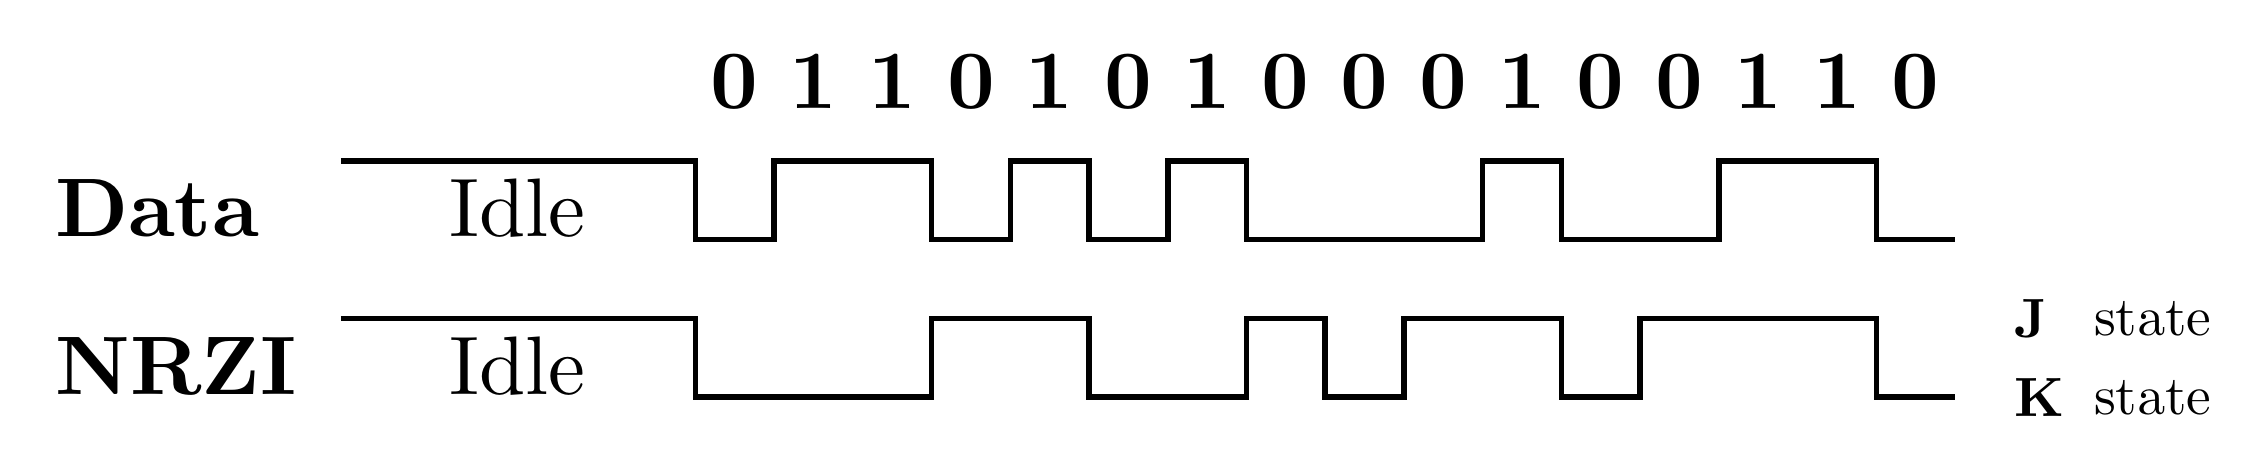
\begin{tikzpicture}

\node[scale=3] at (0, 0) {\bf 0};
\node[scale=3] at (1, 0) {\bf 1};
\node[scale=3] at (2, 0) {\bf 1};
\node[scale=3] at (3, 0) {\bf 0};
\node[scale=3] at (4, 0) {\bf 1};
\node[scale=3] at (5, 0) {\bf 0};
\node[scale=3] at (6, 0) {\bf 1};
\node[scale=3] at (7, 0) {\bf 0};
\node[scale=3] at (8, 0) {\bf 0};
\node[scale=3] at (9, 0) {\bf 0};
\node[scale=3] at (10, 0) {\bf 1};
\node[scale=3] at (11, 0) {\bf 0};
\node[scale=3] at (12, 0) {\bf 0};
\node[scale=3] at (13, 0) {\bf 1};
\node[scale=3] at (14, 0) {\bf 1};
\node[scale=3] at (15, 0) {\bf 0};

\path[draw, line width=2] (-5, -1) -- ++(4.5, 0)
            -- ++(0, -1) -- ++(1, 0)
            -- ++(0, 1)  -- ++(1, 0)
                         -- ++(1, 0)
            -- ++(0, -1) -- ++(1, 0)
            -- ++(0, 1)  -- ++(1, 0)
            -- ++(0, -1) -- ++(1, 0)
            -- ++(0, 1)  -- ++(1, 0)
            -- ++(0, -1) -- ++(1, 0)
                         -- ++(1, 0)
                         -- ++(1, 0)
            -- ++(0, 1)  -- ++(1, 0)
            -- ++(0, -1) -- ++(1, 0)
                         -- ++(1, 0)
            -- ++(0, 1)  -- ++(1, 0)
                         -- ++(1, 0)
            -- ++(0, -1) -- ++(1, 0);

\path[draw, line width=2] (-5, -3) -- ++(4.5, 0)
            -- ++(0, -1) -- ++(1, 0)
                         -- ++(1, 0)
                         -- ++(1, 0)
            -- ++(0, 1)  -- ++(1, 0)
                         -- ++(1, 0)
            -- ++(0, -1) -- ++(1, 0)
                         -- ++(1, 0)
            -- ++(0, 1)  -- ++(1, 0)
            -- ++(0, -1) -- ++(1, 0)
            -- ++(0, 1)  -- ++(1, 0)
                         -- ++(1, 0)
            -- ++(0, -1) -- ++(1, 0)
            -- ++(0, 1)  -- ++(1, 0)
                         -- ++(1, 0)
                         -- ++(1, 0)
            -- ++(0, -1) -- ++(1, 0);

\node[anchor=west,scale=2] at (16, -3) {\bf J};
\node[anchor=west,scale=2] at (16, -4) {\bf K};
\node[anchor=east,scale=2] at (19, -3) {state};
\node[anchor=east,scale=2] at (19, -4) {state};
\node[anchor=west,scale=3] at (-4, -1.6) {Idle};
\node[anchor=west,scale=3] at (-4, -3.6) {Idle};
\node[anchor=west,scale=3] at (-9, -1.6) {\bf Data};
\node[anchor=west,scale=3] at (-9, -3.6) {\bf NRZI};

\end{tikzpicture}

}
\end{figure}

For keeping the receiver clock in sync with the data it is not ideal if the signal
stays at J or K for too long. To prevent this, a technique called "bit stuffing"
is used: Before doing NRZI encoding, a zero is inserted after every six consecutive ones
in the data. The receiver recognizes the stuffed bits during decoding and discards them
\cite[p. 157]{usbstd}.

\subsection {Packets}

Packets are the atomic unit of data transmission in USB. In between packet transmission,
the bus remains in an idle state. Every packet starts with a sync pattern to synchronize
the clocks between sender and receiver. Next are the actual data bits. The packet is
terminated by an EOP state. Fields in a packet are transmitted least-significant
bit first \cite[p. 195]{usbstd}.

The first 8 bits of every packet contain the packet ID (PID) which identifies its type
and thus how the rest of the packet data should be interpreted. The PID is 4 bits long,
they are transmitted a second time in reverse bit order to allow the receiver to quickly
discard a faulty packet. There are 17 different packet types (PRE and ERR have the same ID,
some are only relevant for High Speed) \cite[p. 195]{usbstd}:

\begin{table}[H]
  \caption{USB packet types; notice how the least-significant two bits identify the packet category \cite[p. 196]{usbstd}}
  \centering
  \begin{tabularx}{\textwidth}{l | l | l | X}
    PID type & PID name & \begin{tabular}{@{}l} PID bits \\ (3..0) \end{tabular} & Description \\ \hline
    \multirow{4}*{Token} & OUT & 0001 & Address + endpoint number for host-to-device transaction \\
                         & IN & 1001 & Address + endpoint number for device-to-host transaction \\
                         & SOF & 0101 & Start-of-frame marker, frame number \\
                         & SETUP & 1101 & Special host-to-device transaction for device configuration \\ \hline
    \multirow{4}*{Data} & DATA0 & 0011 & Data packet \\
                         & DATA1 & 1011 & Data packet \\
                         & DATA2 & 0111 & Data packet (only High Speed) \\
                         & MDATA & 1111 & Data packet (only High Speed) \\ \hline
    \multirow{4}*{Handshake} & ACK & 0010 & Receiver accepts error-free data packet \\
                         & NAK & 1010 & Receiver cannot accept data or transmitter cannot send data \\
                         & STALL & 1110 & Endpoint halted or control pipe request not supported \\
                         & NYET & 0110 & Data packet (only High Speed) \\ \hline
    \multirow{4}*{Special} & PRE & 1100 & Preamble to enable downstream traffic to low-speed devices \\
                         & ERR & 1100 & Split Transaction error handshake \\
                         & SPLIT & 1000 & High speed Split Transaction token (only High Speed) \\
                         & PING & 0100 & High speed control flow probe (only High Speed) \\
                         & Reserved & 0000 & Reserved PID \\
  \end{tabularx}
\end{table}

\subsubsection{Token packet}

\begin{figure}[H]
  \caption{Token packet format (after \cite[p. 199]{usbstd})}
  \centering
  \scalebox{1}{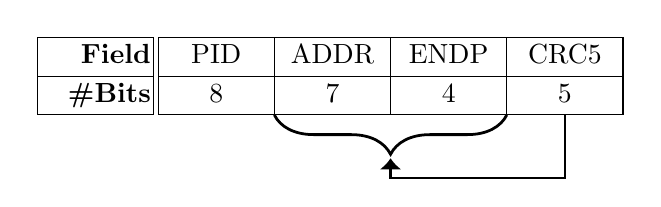
\begin{tikzpicture}
\matrix (M)
[
  matrix of nodes,
  row sep = -\pgflinewidth,
  column sep = -\pgflinewidth,
  nodes = {
    inner sep=1,
    outer sep=0,
    draw,
    text height = \ht\strutbox,
    text depth = \dp\strutbox,
    minimum width = 32,
    minimum height = 5,
    text width = 40,
    align=center
  },
  column 1/.style = {column sep = 3\pgflinewidth,nodes={align=right}},
]
{
  \bf Field & PID & ADDR & ENDP & CRC5 \\
  \bf \#Bits & 8 & 7 & 4 & 5 \\
};

\coordinate(A) at (M-2-3.south west);
\coordinate(B) at (M-2-4.south east);
\coordinate(S) at (M-2-5.south);
\coordinate(C) at ($0.5*(A) + 0.5*(B) + (0, -5.5mm)$);
\path[line width=1, draw, decorate, decoration={brace, amplitude=5mm, mirror}] (A) -- (B);
\draw[-{Latex[width=8,length=4]}, line width=1] (S) -- ++(0, -0.8) -| (C);
\end{tikzpicture}
}
  \label{fig:tokenpacket}
\end{figure}

Token packets (\autoref{fig:tokenpacket}) are used at the start of so-called transactions to specify the target
of the transaction on the bus, namely a certain device and endpoint. There are 127
possible devices on a bus (address 0 is reserved for a device that has not been configured yet).
\cite[p. 256]{usbstd}

Endpoints are logical entities on a device that are used as sources and sinks of data
in so-called pipes. A pipe is either in OUT (to device) or IN (to host) direction.
Endpoint 0 is a special bidirectional pipe that must be available on every device
right after the reset. It is used mainly for identifying and configuring the device.
\cite[p. 33]{usbstd}

A 5-bit checksum validates the endpoint and address information.

\subsubsection{Data packet}

\begin{figure}[H]
  \caption{Data packet format (after \cite[p. 206]{usbstd})}
  \centering
  \scalebox{1}{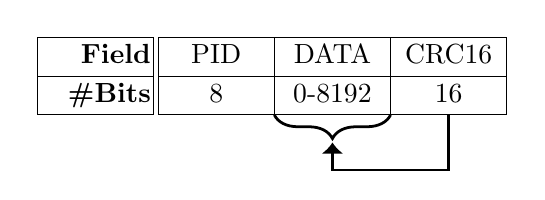
\begin{tikzpicture}
\matrix (M)
[
  matrix of nodes,
  row sep = -\pgflinewidth,
  column sep = -\pgflinewidth,
  nodes = {
    inner sep=1,
    outer sep=0,
    draw,
    text height = \ht\strutbox,
    text depth = \dp\strutbox,
    minimum width = 32,
    minimum height = 5,
    text width = 40,
    align=center
  },
  column 1/.style = {column sep = 3\pgflinewidth,nodes={align=right}},
]
{
  \bf Field & PID & DATA & CRC16 \\
  \bf \#Bits & 8 & 0-8192 & 16 \\
};

\coordinate(A) at (M-2-3.south west);
\coordinate(B) at (M-2-3.south east);
\coordinate(S) at (M-2-4.south);
\coordinate(C) at ($0.5*(A) + 0.5*(B) + (0, -3.5mm)$);
\path[line width=1, draw, decorate, decoration={brace, amplitude=3mm, mirror}] (A) -- (B);
\draw[-{Latex[width=8,length=4]}, line width=1] (S) -- ++(0, -0.7) -| (C);
\end{tikzpicture}
}
\end{figure}

Used to transmit the actual data in a transaction.
A 16-bit checksum validates the transmitted data.

\subsubsection{Handshake packet}

\begin{figure}[H]
  \caption{Handshake packet format (after \cite[p. 206]{usbstd})}
  \centering
  \scalebox{1}{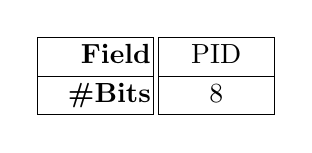
\begin{tikzpicture}
\matrix (M)
[
  matrix of nodes,
  row sep = -\pgflinewidth,
  column sep = -\pgflinewidth,
  nodes = {
    inner sep=1,
    outer sep=0,
    draw,
    text height = \ht\strutbox,
    text depth = \dp\strutbox,
    minimum width = 32,
    minimum height = 5,
    text width = 40,
    align=center
  },
  column 1/.style = {column sep = 3\pgflinewidth,nodes={align=right}},
]
{
  \bf Field & PID \\
  \bf \#Bits & 8 \\
};
\end{tikzpicture}

}
\end{figure}

Used to report the status of a transaction.

\subsection{Transfers}

Transfers (\autoref{fig:usbtransfer}) are the abstraction level of data exchange as seen at the software
side of the host. From the host's perspective, a transfer transmits a string of
 bytes from / to the device. A transfer is directed to one of the device's endpoints,
each of them has one of four transfer types plus a transfer direction
associated with it during device configuration.
Transfers are composed of transactions, which usually consist of three
packets \cite[p. 209ff.]{usbstd}:

\begin{enumerate}
  \item A token packet to tell the type of the transaction and its destination
        (as all USB communication is initiated by the host, the token packet always comes
        from the host)
  \item A DATA packet for the actual payload. Length can vary between 8-64 bytes on Full Speed links.
        This can go host to device or device to host.
  \item A handshake packet (usually ACK, NAK) lets the sender know if the data was received successfully.
\end{enumerate}

Transfers usually consist of multiple transactions.

\begin{figure}[H]
  \caption{Composition of a USB transfer (after \cite[p. 44]{uc}).}
  \centering
  \scalebox{1}{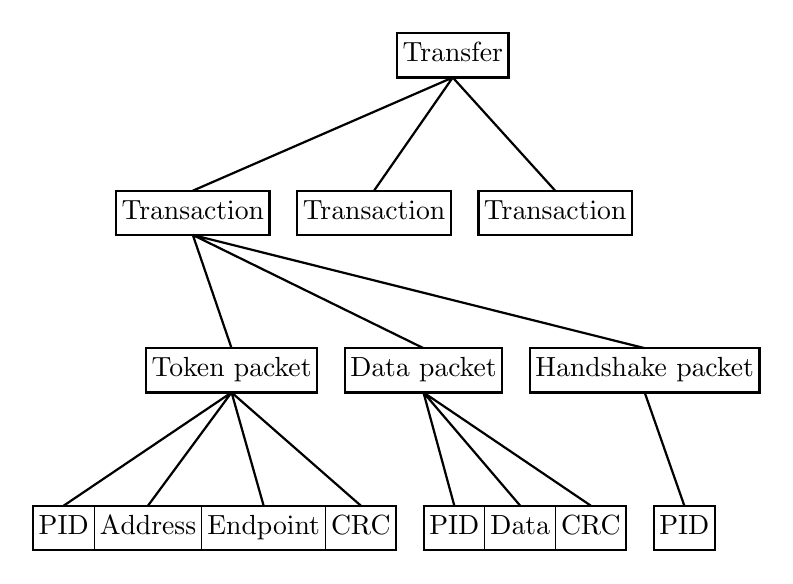
\begin{tikzpicture}
\pgfdeclarelayer{background}
\pgfsetlayers{background,main}

\def\rounding {0}

\tikzset{mstyle/.style={
  matrix of nodes,
  inner sep=2,
  outer sep=0,
  text height=\ht\strutbox,
  text depth=\dp\strutbox
}}

\matrix (M1) at (1, 0) [style=mstyle] {
  Transfer\\
};

\matrix (M2) at (0, -2) [style=mstyle] {
  Transaction & [10] Transaction & [10] Transaction \\
};

\matrix (M3) at (1, -4) [style=mstyle] {
  Token packet & [10] Data packet & [10] Handshake packet \\
};

\matrix (M4) at (0, -6) [style=mstyle] {
  PID & Address & Endpoint & CRC & [10] PID & Data & CRC & [10] PID \\
};

\draw[thick]
  (M1-1-1.south) -- (M2-1-1.north)
  (M1-1-1.south) -- (M2-1-2.north)
  (M1-1-1.south) -- (M2-1-3.north)
  (M2-1-1.south) -- (M3-1-1.north)
  (M2-1-1.south) -- (M3-1-2.north)
  (M2-1-1.south) -- (M3-1-3.north)
  (M3-1-1.south) -- (M4-1-1.north)
  (M3-1-1.south) -- (M4-1-2.north)
  (M3-1-1.south) -- (M4-1-3.north)
  (M3-1-1.south) -- (M4-1-4.north)
  (M3-1-2.south) -- (M4-1-5.north)
  (M3-1-2.south) -- (M4-1-6.north)
  (M3-1-2.south) -- (M4-1-7.north)
  (M3-1-3.south) -- (M4-1-8.north);

\begin{pgfonlayer}{background}
  \def \framepath {
    (M1-1-1.north west) -- (M1-1-1.north east) -- (M1-1-1.south east) -- (M1-1-1.south west) -- cycle
    (M2-1-1.north west) -- (M2-1-1.north east) -- (M2-1-1.south east) -- (M2-1-1.south west) -- cycle
    (M2-1-2.north west) -- (M2-1-2.north east) -- (M2-1-2.south east) -- (M2-1-2.south west) -- cycle
    (M2-1-3.north west) -- (M2-1-3.north east) -- (M2-1-3.south east) -- (M2-1-3.south west) -- cycle
    (M3-1-1.north west) -- (M3-1-1.north east) -- (M3-1-1.south east) -- (M3-1-1.south west) -- cycle
    (M3-1-2.north west) -- (M3-1-2.north east) -- (M3-1-2.south east) -- (M3-1-2.south west) -- cycle
    (M3-1-3.north west) -- (M3-1-3.north east) -- (M3-1-3.south east) -- (M3-1-3.south west) -- cycle
    (M4-1-1.north west) -- (M4-1-4.north east) -- (M4-1-4.south east) -- (M4-1-1.south west) -- cycle
    (M4-1-5.north west) -- (M4-1-7.north east) -- (M4-1-7.south east) -- (M4-1-5.south west) -- cycle
    (M4-1-8.north west) -- (M4-1-8.north east) -- (M4-1-8.south east) -- (M4-1-8.south west) -- cycle
  }

  %~ \begin{scope}
    %~ \clip[rounded corners = \rounding] \framepath;
    %~ \fill[gray!20] (M1-1-1.north west) rectangle (M1-1-1.south east);
    %~ \fill[purple!20] (M2-1-1.north west) rectangle (M2-1-1.south east);
    %~ \fill[purple!20] (M2-1-2.north west) rectangle (M2-1-2.south east);
    %~ \fill[purple!20] (M2-1-3.north west) rectangle (M2-1-3.south east);
    %~ \fill[lime!20] (M3-1-1.north west) rectangle (M3-1-1.south east);
    %~ \fill[orange!20] (M3-1-2.north west) rectangle (M3-1-2.south east);
    %~ \fill[olive!20] (M3-1-3.north west) rectangle (M3-1-3.south east);
    %~ \fill[yellow!20] (M4-1-1.north west) rectangle (M4-1-1.south east);
    %~ \fill[red!20] (M4-1-2.north west) rectangle (M4-1-2.south east);
    %~ \fill[green!20] (M4-1-3.north west) rectangle (M4-1-3.south east);
    %~ \fill[blue!20] (M4-1-4.north west) rectangle (M4-1-4.south east);
    %~ \fill[yellow!20] (M4-1-5.north west) rectangle (M4-1-5.south east);
    %~ \fill[teal!20] (M4-1-6.north west) rectangle (M4-1-6.south east);
    %~ \fill[blue!20] (M4-1-7.north west) rectangle (M4-1-7.south east);
    %~ \fill[yellow!20] (M4-1-8.north west) rectangle (M4-1-8.south east);
  %~ \end{scope}
  
  \draw (M4-1-1.north east) -- (M4-1-1.south east)
        (M4-1-2.north east) -- (M4-1-2.south east)
        (M4-1-3.north east) -- (M4-1-3.south east)
        (M4-1-5.north east) -- (M4-1-5.south east)
        (M4-1-6.north east) -- (M4-1-6.south east);

  \draw[thick, rounded corners = \rounding] \framepath;
\end{pgfonlayer}

\end{tikzpicture}
}
  \label{fig:usbtransfer}
\end{figure}

\subsubsection {Control transfer}

Every device must have endpoint 0 for control transfers. Control endpoints
are message-based. This means each transfer is for a specific message which has
defined length, format and purpose. There can be transfers in either direction
on the same endpoint, although each transfer has a specified (data stage) direction.
Control transfers start with a Setup stage / transaction specifying the target device
and endpoint plus an extra 8 bytes of data called the Device Request \cite[p. 38f.]{usbstd}.

\begin{table}[H]
  \caption{Device Request format \cite[p. 248]{usbstd}}
  \centering
  \begin{tabularx}{\textwidth}{l | l | l | X}
    \begin{tabular}{@{}l} Offset \\ (bytes) \end{tabular} & Field &
    \begin{tabular}{@{}l} Size \\ (bytes) \end{tabular} & Description \\ \hline
    
    0 & bmRequestType & 1 &
    
      Bits 0..4: Recipient
      
      \begin{tabular}{l l}
        0 & Device \\
        1 & Interface \\
        2 & Endpoint \\
        3 & Other \\
        4..31 & Reserved \\
      \end{tabular}
      
      \vspace{3mm}
      Bits 5..6: Type
      
      \begin{tabular}{l l}
        0 & Standard \\
        1 & Class \\
        2 & Vendor \\
        3 & Reserved \\
      \end{tabular}
      
      \vspace{3mm}
      Bit 7: Transfer direction
      
      \begin{tabular}{l l}
        0 & Host to device \\
        1 & Device to host \\
      \end{tabular} \\ \hline
  
    1 & bRequest & 1 & Specific request \\ \hline
    2 & wValue & 2 & Varies according to request \\ \hline
    4 & wIndex & 1 & Varies according to request, typically used
    for a index or offset \\ \hline
    6 & wLength & 2 & Number of bytes to be transferred in the data stage
    (0 means no data stage) \\
  \end{tabularx}
  \label{table:ctrltransfer}
\end{table}

Depending on the kind of control transfer, there may be a data stage
consisting of data transactions, but this is not required. If there
are data transactions, all are going in the same direction as specified
by the request type.
The transfer is completed with a Status transaction to report back
about the success of the whole transfer.

Control transfers are used right after the device reset to get information about
its capabilities and set a configuration. For this, there are 11 bRequest values
called Standard Requests that have to be supported by all devices as part of the standard.

\begin{table}[H]
  \caption{Some important Standard Requests \cite[p. 250]{usbstd}}
  \centering
  \begin{tabularx}{\textwidth}{l | l | X | X}
    bRequest & \begin{tabular}{@{}l}  bmRequestType \\ (7..0) \end{tabular}
     & wValue & wIndex \\ \hline
    
    GET\_DESCRIPTOR & 10000000 & Descriptor type and index & Zero or Language ID \\ \hline
    SET\_ADDRESS & 00000000 & Device address & Zero \\ \hline
    GET\_STATUS & \begin{tabular}{@{}l}  10000000 \\ 10000001 \\ 10000010 \end{tabular}
    & Zero & \begin{tabular}{@{}l}  Zero \\ Interface \\ Endpoint \end{tabular} \\ \hline
    SET\_CONFIGURATION & 00000000 & Configuration value & Zero \\
  \end{tabularx}
  
  \vspace{5mm}
  \begin{tabularx}{\textwidth}{l | l | X}
    bRequest & wLength & Data \\ \hline
    
    GET\_DESCRIPTOR & Descriptor length & Descriptor \\
    SET\_ADDRESS & None & None \\
    GET\_STATUS & Two & Device, Interface or endpoint status \\
    SET\_CONFIGURATION & None & None \\
  \end{tabularx}
\end{table}

They are also used to control the device after the configuration phase during normal operation.
There are standardized requests (Class Requests) for certain device classes like keyboards, storage devices etc.

Other non-standard devices have custom, vendor-specific requests that are not documented
in the USB standard.

\subsubsection {Bulk transfer}

Bulk transfers are used to transmit large amounts of data with guaranteed delivery
and low overhead but no latency / bandwidth constraints.
Compared to control transfers, they are stream-based. This means there is no defined message
format or size. For an IN endpoint, the host would poll the device endpoint for data until it receives
(cumulative) as many bytes as requested by the software. A transfer can also be ended by the device sending
a data transaction of less size than the maximum of this endpoint (data is always split so there is at most one
smaller packet at the end) or a zero-size data transaction. To avoid data packets being lost, they
alternate between the DATA0 / DATA1 PIDs. A single bulk endpoint is only for incoming
or only for outgoing transfers.
The host schedules them at times when the bus bandwidth is not used by other transfer types.
Typical uses for bulk transfers are transferring data from/to an external hard disk,
to a printer or from a scanner. \cite[p. 52ff.]{usbstd}

\subsubsection {Interrupt transfer}

On the bus, interrupt transfers look the same as bulk transfers.
The main difference is scheduling: The host guarantees that a transfer
attempt is made as often as specified in the endpoint descriptor (1 - 100 ms).
Despite the name, interrupt transfers have nothing to do with hardware interrupts.
All communication on the USB bus is initiated by the host, so it has to poll the device
for data.
Typical uses for interrupt transfers are receiving key presses from keyboards and
movements from mice \cite[p. 48ff.]{usbstd}.

\subsubsection {Isochronous transfer}

Isochronous transfers are for transmitting data at a constant rate with guaranteed
latency. Compared to interrupt transfers, they offer a guaranteed transfer rate
(with interrupt transfers the interval between two transfers can be anywhere
between zero and the specified maximum). The drawback is a lack of any handshake
/ retry mechanism.
Typical uses for isochronous transfers are USB sound cards or webcams
\cite[p. 44ff.]{usbstd}.

\subsection{Device initialization}
\label{devinit}

The process from a device being plugged in to it becoming usable for the user
roughly goes as follows (every USB bus has at least a root hub device interacting with
the operating system) \cite[p. 87ff.]{uc}:

\begin{enumerate}
  \item The hub detects the device by the change in levels on the data lines.
  \item The hub reports the device to the host.
  \item The host tells the hub to reset the device so communication can begin.
  \item The host assigns an address to the new device.
  \item The host asks for the Device Descriptor to get information identifying the device
        (vendor / product ID, device class).
  \item The host looks for a driver handling this VID / PID combination, if it does not find one,
        it leaves the device in an unconfigured state.
  \item If a driver is found, it is loaded. The device is asked for its configuration profiles.
        The driver sets a configuration and can now make the device serve its purpose.
\end{enumerate}

\subsubsection{Device descriptor}

After setting the address, a GET\_DESCRIPTOR
device request is made, asking for the device descriptor.

\begin{table}[H]
  \caption{Device descriptor format \cite[p. 262f.]{usbstd}}
  \centering
  \begin{tabularx}{\textwidth}{l | l | l | X}
    \begin{tabular}{@{}l} Offset \\ (bytes) \end{tabular} & Field &
    \begin{tabular}{@{}l} Size \\ (bytes) \end{tabular} & Description \\ \hline
    
    0 & bLength & 1 & Descriptor size in bytes \\
    1 & bDescriptorType & 1 & 1 for DEVICE descriptor \\
    2 & bcdUSB & 2 & USB specification release number \\
    4 & bDeviceClass & 1 & Class code \\
    5 & bDeviceSubclass & 1 & Subclass code \\
    6 & bDeviceProtocol & 1 & Protocol code \\
    7 & bMaxPacketSize0 & 1 & Maximum packed size for Endpoint 0  \\
    8 & idVendor & 2 & Vendor ID \\
    10 & idProduct & 2 & Product ID \\
    12 & bcdDevice & 2 & Device release number \\
    14 & iManufacturer & 1 & Index of manufacturer string descriptor \\
    15 & iProduct & 1 & Index of product string descriptor \\
    16 & iSerialNumber & 1 & Index of serial number string descriptor \\
    17 & bNumConfigurations & 1 & Number of possible configurations \\
  \end{tabularx}
\end{table}


{\bf bDeviceClass} Classes are types of devices that were standardized in USB.
There are class codes for audio devices, human interface devices, storage devices etc.
There is also a vendor-specific class code for devices not conforming to a standardized class.
They are further divided into subclasses specifying the actual functionality more
precisely (i.e. keyboard vs. mouse for HID device).

{\bf idVendor} is a 16-bit identifier assigned by the USB Implementers Forum
for each manufacturer of USB compliant devices. Manufacturers must apply
for a unique ID there.

{\bf idProduct} is a 16-bit identifier assigned by the manufacturer
of the device. Manufacturers manage their own PID space so that IDs
are unique per device.



\subsubsection{Configuration descriptor}

Configurations are profiles that define one or more interfaces for the device
and their characteristics.
Only one configuration can be active at a time \cite[p. 244]{usbstd}.

\begin{table}[H]
  \caption{Configuration descriptor format \cite[p. 265]{usbstd}.}
  \centering
  \begin{tabularx}{\textwidth}{l | l | l | X}
    \begin{tabular}{@{}l} Offset \\ (bytes) \end{tabular} & Field &
    \begin{tabular}{@{}l} Size \\ (bytes) \end{tabular} & Description \\ \hline
    
    0 & bLength & 1 & Descriptor size in bytes \\
    1 & bDescriptorType & 1 & 2 for CONFIGURATION descriptor \\
    2 & wTotalLength & 2 & Total length of all descriptors for this configuration \\
    4 & bNumInterfaces & 1 & Number of interfaces in this configuration \\
    5 & bConfigurationValue & 1 & Value to be used to select this configuration with SET\_CONFIGURATION \\
    6 & iConfiguration & 1 & Index of string descriptor for this configuration \\
    7 & bmAttributes & 1 & Bitmap of configuration characteristics (Self-powered etc.) \\
    8 & bMaxPower & 1 & Maximum power consumption from bus in this configuration (mA) \\
  \end{tabularx}
\end{table}

\subsubsection{Interface descriptor}

Interfaces are sets of related endpoints that together provide a certain feature
of the device. Devices can have multiple active interfaces at the same time.
Additionally, interfaces can have alternate settings that change its endpoints' characteristics
\cite[p. 244]{usbstd}.

Device drivers are often assigned to serve a specific interface rather than an entire device.

\begin{table}[H]
  \caption{Interface descriptor format \cite[p. 268f.]{usbstd}}
  \centering
  \begin{tabularx}{\textwidth}{l | l | l | X}
    \begin{tabular}{@{}l} Offset \\ (bytes) \end{tabular} & Field &
    \begin{tabular}{@{}l} Size \\ (bytes) \end{tabular} & Description \\ \hline

    0 & bLength & 1 & Descriptor size in bytes \\
    1 & bDescriptorType & 1 & 4 for INTERFACE descriptor \\
    2 & bInterfaceNumber & 1 & Number identifying this interface \\
    3 & bAlternateSetting & 1 & Value specifying alternate setting for this interface \\
    4 & bNumEndpoints & 1 & Number of endpoints in this interface (excluding default endpoint 0) \\
    5 & bInterfaceClass & 1 & Type of functionality provided by interface (similar to Device class) \\
    6 & bInterfaceSubClass & 1 & Subclass of device type (similar to Device class) \\
    7 & bInterfaceProtocol & 1 & Protocol of class-specific requests made for this interface \\
    8 & iInterface & 1 & Index of string descriptor for this interface \\
  \end{tabularx}
\end{table}

\subsubsection{Endpoint descriptor}

Endpoint descriptors specify an endpoint's address, type, and polling interval.

\begin{table}[H]
  \caption{Endpoint descriptor format \cite[p. 269ff.]{usbstd}}
  \centering
  \begin{tabularx}{\textwidth}{l | l | l | X}
    \begin{tabular}{@{}l} Offset \\ (bytes) \end{tabular} & Field &
    \begin{tabular}{@{}l} Size \\ (bytes) \end{tabular} & Description \\ \hline
    0 & bLength & 1 & Descriptor size in bytes \\
    1 & bDescriptorType & 1 & 5 for ENDPOINT descriptor \\
    2 & bEndpointAddress & 1 & Bits 3..0 give endpoint number, bit 7 gives endpoint direction
        (0 - out, 1 - in) \\
    3 & bmAttributes & 1 & Bits 1..0 describe endpoint type (Control, Isochronous, Bulk, Interrupt).
        Bits 5..2 specify extra options for isochronous endpoints \\
    4 & wMaxPacketSize & 2 & maximum packet size of the endpoint \\
    6 & bInterval & 1 & How often the host should poll for data (in microframes)
  \end{tabularx}
\end{table}

\subsubsection{String descriptor}

String descriptors provide information about the device in human-readable form.
String descriptor 0 transmits language codes supported by the device.

\begin{table}[H]
  \caption{String descriptor format \cite[p. 273f.]{usbstd}}
  \centering
  \begin{tabularx}{\textwidth}{l | l | l | X}
    \begin{tabular}{@{}l} Offset \\ (bytes) \end{tabular} & Field &
    \begin{tabular}{@{}l} Size \\ (bytes) \end{tabular} & Description \\ \hline
    0 & bLength & 1 & Descriptor size in bytes \\
    1 & bDescriptorType & 1 & for STRING descriptor \\
    2 & bString & rest & String, UNICODE encoded
  \end{tabularx}
\end{table}

\section{USB sniffing}

USB sniffing is the process of recording communication on the USB bus.
This is useful for device developers, driver developers, keyloggers etc.

\subsection{Hardware vs. software sniffing}
\label{ssec:snifferscompared}

Hardware sniffing uses a dedicated device that sits on the bus in between the
host and device. Dedicated software is used to interpret the low-level signals
as packets / transactions.

Software sniffing does not use dedicated hardware to listen to the signals
on the wires. Instead, the host operating system reports packets sent / received
to some software running on the same host.

\paragraph*{Advantages of hardware USB analyzers \cite{analyzerbenefits}}:

\begin{itemize}
\item Independent of the host, not affected by bugs in its USB hardware / software
\item Allow analysis down to the lowest level (voltage levels between wires)
\item See all packets transmitted, including unsuccessful transactions etc.
\end{itemize}

\paragraph*{Advantages of purely software USB analyzers:}

\begin{itemize}
\item Lower cost (free when using usbmon / Wireshark)
\item Easy setup, convenient, no extra hardware required
\end{itemize}

\subsection{usbmon}

{\it usbmon} is a module for the Linux kernel that allows access to
USB request blocks (URBs) as they are being processed. URBs are a
data structure of the Linux kernel and loosely correspond to USB transfers. \cite{usbmon}

\subsubsection{Payload size limitation}

An interesting pitfall when using {\it usbmon} is that for URBs with a payload
longer than 61440 bytes only the first 61440 are captured, the rest is truncated.
Others have faced this problem, unsure where it comes from and what to do: \cite{usbmon_others}

\begin{figure}[H]
  \caption{A large bulk transfer in Wireshark, {\it Data length} $<$ {\it URB length}
           indicates missing bytes.}
  \centering
  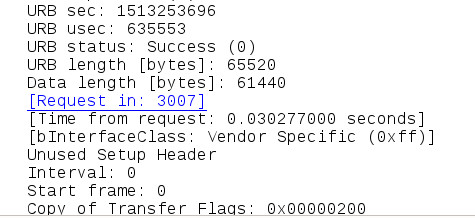
\includegraphics[width=0.8\textwidth]{images/jpg/usbmon_wireshark.jpg}
\end{figure}

\begin{figure}[H]
  \caption{Image reconstructed from payloads. The frequent tearing is caused by the large
  65520 byte transfers being truncated to 61440 bytes.}
  \centering
  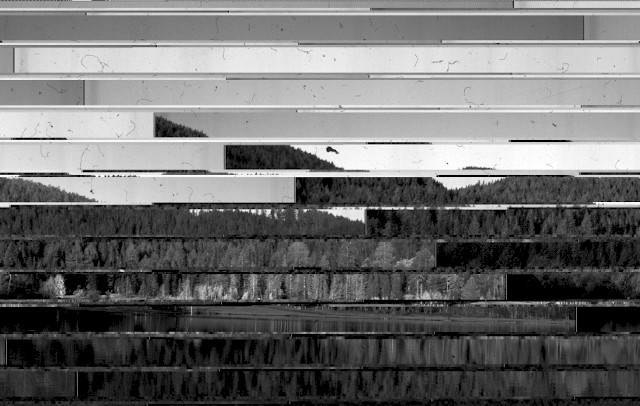
\includegraphics[width=0.8\textwidth]{images/jpg/usbmon_chopped.jpg}
\end{figure}

\subsubsection{Kernel patching}
\label{ssec:kernelpatch}

Since the problem persisted when changing computers, sniffing software and target devices
it was concluded it must be in the {\it usbmon} kernel module itself.
The {\it linux-source} package (kernel version 4.13) was installed on the {\it Debian 9} system.

Source code for {\it usbmon} is found in {\it drivers/usb/mon}. {\it usbmon} has a
text-based and a binary interface. The binary interface is used by external sniffing
software like Wireshark. The code for it is in {\it mon\_bin.c}.

The magic limit 61440 was not found in the code. However the {\it mon\_bin\_event} procedure
which is involved in extracting data from a current kernel USB event has an interesting statement: \\
\verb|    if (length >= rp->b_size/5) length = rp->b_size/5; |. \\
The default buffer size (this value lands in \verb|rp->b_size|) is defined as \\
\verb|    #define BUFF_DFL   CHUNK_ALIGN(300*1024) |. \\
This gives a maximum length of $\frac{300*1024}{5} = 61440$. Data payloads less
than one fifth of the buffer size are truncated for unknown reasons.
This line was changed to remove the limitation: \\
\verb|    if (length >= rp->b_size) length = rp->b_size; |. \\
The modified kernel was compiled and installed according to standard Debian procedures \cite{debkernel}.
When running this kernel, the full 65520 bytes of payload could be captured.
No adverse side effects were noticed.

\subsection{Wireshark}
\label{ssec:wireshark}

Wireshark \cite{wireshark} is a cross-platform sniffing and packet analysis software that
became famous as an Ethernet (network) traffic sniffer.
It can be used both for recording traffic as well as analyzing it.
For analyzing, it comes with many protocol dissectors that subsequently
decode the layers of the packet giving a readable description of the protocol fields'
values and their meaning.

Also part of Wireshark is the {\it tshark} \cite{wireshark_tshark} utility. It is basically
a command-line version of Wireshark, also accessing
the same configuration files, this means behavior of {\it tshark} can be configured
inside Wireshark, for instance which protocols are enabled. {\it tshark} is ideal for scripts
that need to parse the {\it .pcapng} capture files generated by Wireshark.
Packets can be filtered by field values and only the desired fields printed.

Wireshark version 2.2.6 was used, other versions may be significantly different.

\subsubsection{Steps}
\label{sniffingprocess}

\begin{enumerate}
  \item Find the bus the device is on using the {\it lsusb} command.
        Ideally, make sure there are no other devices
        on this bus (except the root hub). Try to plug it into different ports.
  
  \item Load the {\it usbmon} kernel module. ({\it modprobe usbmon} as root)
  
  \item Launch {\it wireshark} as root.
  
  \item Select the {\it usbmon*} input corresponding to the bus found in Step 1 and press Start.
  
  \item When completed, stop the recording and save to disk.
  \end{enumerate}

\subsubsection{Customize columns}

For USB sniffing, it is useful to have the most important packet fields as columns.
This allows a good insight into the data flow at a certain time when scrolling through the packet list.
Also, packets can be sorted using some column, allowing them to be grouped according to endpoint,
payload length etc. 

To manage columns, go to {\it Edit $\,\to\,$ Preferences $\,\to\,$ Columns}. New columns are best added
by right clicking on the desired field in the analysis window and selecting "Apply as column".

A good selection of columns could be:
Packet number, Time, Source, Destination,
Length, Info, Leftover capture data ({\it usb.capdata}).
For going through long sequences of control transfers, columns for the control transfer parameters
({\it bmRequestType, bRequest, wValue, wIndex, Data fragment}) are helpful.

\subsubsection{Disable non-USB protocols}
\label{nonusb}

For USB sniffing, none of the supplied protocol dissectors except USB are helpful.
Even worse, they can get in the way by seeing the first bytes of the data payload match
some pattern which causes them to be interpreted as some protocol while they are just raw pixel
values. For these packets, the {\it usb.capdata} field becomes unavailable which makes their
payload ignored when parsing the capture file. This leads to missing image bytes, noticeable
as a tear in the image (similar to a truncated payload).

To fix this, go to {Analyze $\,\to\,$ Enabled protocols}, click "Disable all" and
then enable only USB. \cite[Section 10.4]{wireshark_userguide}

\subsection{Example}

\subsubsection{Scenario}

To provide some insight into the sniffing process and how the recorded data can be
interpreted, I chose to record keystrokes from a USB keyboard. Since USB keyboards
are very widespread and follow a standard protocol, the experiment can be repeated
by almost anyone.

A bus with no devices on it (except the mandatory root hub with address 1) is chosen
for sniffing.
Recording is started before the device gets attached.
The keyboard is attached, then the following keys are pressed and
then released (one after another): a, b, a. Recording is then stopped.

For brevity, only a few of the captured packets are discussed here.

\subsubsection{Device configuration}

When the device is connected, a process like in \autoref{devinit} starts.
The device is reset, an address issued and descriptors queried. The device
descriptor and the interface / endpoint descriptor are shown here.

\begin{figure}[H]
  \caption{Device descriptor of USB keyboard}
  \centering
  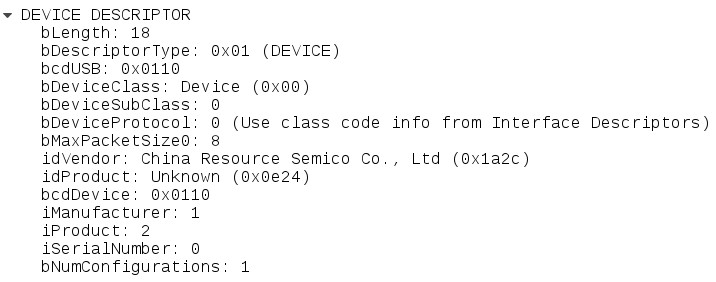
\includegraphics[width=\textwidth]{images/jpg/sniff_keyboard_1.jpg}
\end{figure}

The class code of 00 signifies that information about the device should be
obtained from the interface descriptor. The vendor name is queried
from a database by Wireshark (only the 2 byte ID is transmitted over the bus).

\begin{figure}[H]
  \caption{Interface / endpoint descriptor of USB keyboard}
  \centering
  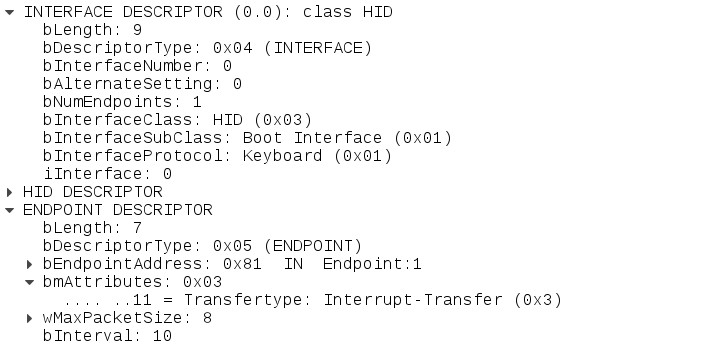
\includegraphics[width=\textwidth]{images/jpg/sniff_keyboard_2.jpg}
\end{figure}

The interface identifies as a keyboard and has one extra input endpoint.
Interrupt transfers should be performed there every 10ms.
The data received from the endpoint is an 8-byte HID report giving information
about pressed keys. The first of these bytes describes pressed modifier keys
(Ctrl, Alt etc.) the second byte is reserved, the third byte describes the
actual pressed key. \cite{usbhid}

\subsubsection{Data transmitted while keys are pressed}

\begin{figure}[H]
  \caption{HID reports from USB keyboard}
  \centering
  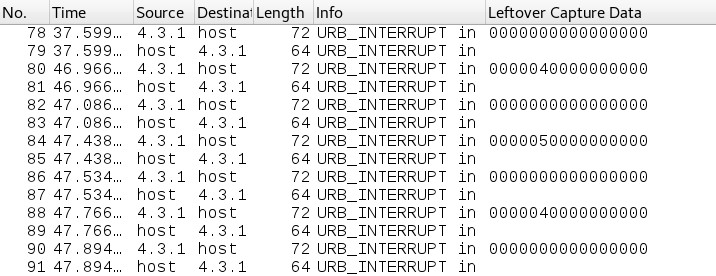
\includegraphics[width=\textwidth]{images/jpg/sniff_keyboard_3.jpg}
\end{figure}

In \cite[p.53]{usbusage} the byte values 04 and 05 stand for the a and
b keys respectively.

\subsection{Sniffing using VirtualBox}
\label{ssec:virtualbox}

When trying to capture device communication from some operating system, it
is convenient to take Linux as a host due to its good sniffing capabilities and
install the target operating system and device driver in a virtual machine.
The virtualization software used here is Oracle VirtualBox \cite{vbox}.

To allow the virtual machine to access the device, the "USB passthrough" feature is used.
This makes the device visible to the guest operating system: VirtualBox
relays communication between the actual device on the host and the virtual device connected
to a virtual USB controller for the guest.
The passthrough is limited to devices with a specified vendor / product ID combination,
new devices can be added by selecting the machine and clicking (Settings $\,\to\,$ USB).

\section{Image extraction}
\label{sec:extract}

As a first step, I wanted to reconstruct the transmitted image from the
sniffed communication during a scan. This is done without interaction between
my own software and the scanner, only the capture file is analyzed. Extracting the
image is also a necessary step when implementing actual scanning software.

\subsection{Setup}

The Windows XP operating system was set up inside VirtualBox. The
vendor-supplied CyberView X5 scanner software \cite{cvx5} (version 5.16) was installed.
The scanner was connected to the VM via USB passthrough.

\begin{figure}[H]
  \caption{CyberView X5 software}
  \centering
  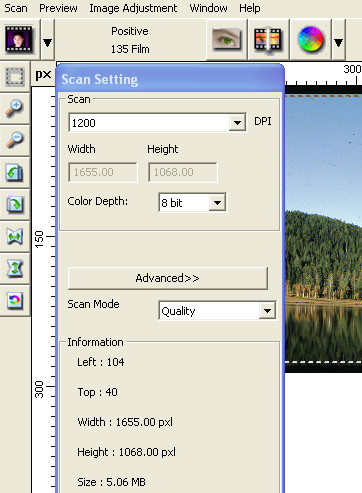
\includegraphics[width=0.75\textwidth]{images/jpg/extract_screenshot.jpg}
\end{figure}

The scanner software was configured to scan a color positive at 1200 dpi resolution.
Digital ICE dust correction was enabled (Scan $\,\to\,$ Preference $\,\to\,$ Positive $\,\to\,$ ICE / ROC / GEM) to make the scanner
record the infrared channel as well.

The scan (Scan $\,\to\,$ Scan) was performed first thing after the software had started so as to
get any kind of calibration data being exchanged only during the first scan.

Wireshark recording was started before starting the scanner software and stopped
after the software had saved the image.

It is important to use a kernel capable of recording the full payload (\autoref{ssec:kernelpatch})
and also to disable extra protocols in Wireshark (\autoref{nonusb}).

A color slide photo of a lake, mountain peaks, green / yellow trees,
reflections in the water and sky was used as target.
It allows one to easily know which channel (when having them as separate grayscale images)
is red, green or blue and provides a good impression of overall image quality.

\subsection{Looking at the capture}

\begin{figure}[H]
  \caption{Large bulk transfers}
  \centering
  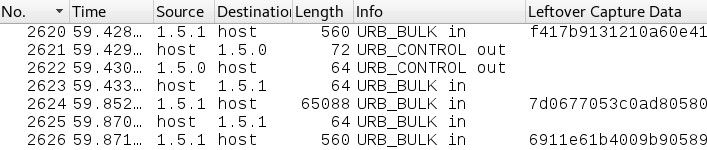
\includegraphics[width=\textwidth]{images/jpg/extract_sniff_1.jpg}
\end{figure}

The scan took about 30 seconds and generated a capture around 18 megabytes
in size. The image saved by the scanner software was 1644 x 1069 pixels large.
When scrolling through the capture, there are many large bulk transfers
incoming from endpoint 1. It seems likely these contain the image data.
Since scanners work on a line-by-line basis and the data is transferred
in small chunks during the scan, the pixels are probably transferred
one line after the other.

\begin{figure}[H]
  \caption{Even (dark) and odd (light) offset bytes of payload}
  \centering
  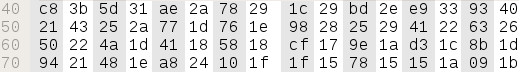
\includegraphics[width=\textwidth]{images/jpg/extract_sniff_2.jpg}
\end{figure}

\label{capture_highlowbytes}

When looking at the payload of one of the transfers, bytes with odd offset
have little variation among their neighbors while those with even offset
seem almost random. This suggests the scanner delivers uncompressed
16 bit per pixel little-endian data:
The odd bytes contain the approximate brightness and
the even bytes the fine nuances (noise).

\subsection{Extraction tool}

Since we are likely dealing with uncompressed line-by-line image data,
it should be possible to construct the image by concatenating the payload bytes
and partitioning them into rows. For this, a Python script {\it extractImage.py} was created,
it performs the following steps:

\begin{enumerate}
  \item Load the {\it .pcapng} file generated by Wireshark using {\it tshark} (option {\it --inputFile}).
        Make {\it tshark} print the payload field ({\it usb.capdata}) as hexadecimal for all
        packets on endpoint 1. Parse and concatenate the lines of {\it tshark}'s output into
        one string of bytes.
  
  \item Apply an offset to the bytes and only keep every n-th (options {\it --byteOffset}, {\it --byteNth}).
        This removes unwanted data at the beginning and only keeps the high byte of the 2 bytes per pixel.
  
  \item Break up the byte string into same-size chunks of a specified size (option {\it --lineLength}),
        each representing a line of the image.

  \item Apply an offset to the lines and only keep every n-th (options {\it --lineOffset}, {\it --lineNth}).
  
  \item Drop all lines beyond a specified maximum (option {\it --lineMax}). This removes abnormal lines at the
        end and brings all color channels to the same dimensions.

  \item Create a grayscale PNG image, dimensions are the line width and the number of remaining lines.
        Write the PNG file (option {\it --outputFile}).
\end{enumerate}

\subsection{Results}
\label{ssec:extract_results}

\begin{figure}[H]
  \caption{Transferred bytes, line width 1644}
  \centering
  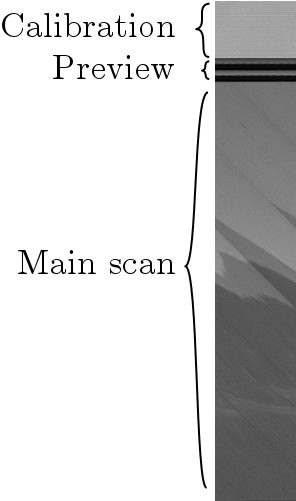
\includegraphics[height=6cm]{images/jpg/extract_sections.jpg}
\end{figure}

The transferred bytes form three distinct images: The first section
is a calibration scan, the second is a low-resolution preview scan and the third (largest)
is the actual 1200 dpi scan. The main scan will be analyzed next,
while the calibration scan is analyzed in \autoref{ssec:calibration}.
The pre-scan is not studied further since its purpose can be served by
doing a low-dpi regular scan.

\subsubsection{Offsets, line width}

To find the exact line width, the guessed line width was incremented / decremented by trial-and-error.
The line width is correct when vertical lines in the image (mountain peaks in this case) no
longer appear distorted. The correct line width was found to be 1645.

Only the high bytes were kept to transform the 16-bit pixel values to 8-bit grayscale (\autoref{capture_highlowbytes}),
this is done with the {\it --byteNth 2} option and a proper {\it --byteOffset}. In this capture,
the high bytes are at even offsets (use trial-and-error), so {\it --byteOffset} must be even to keep
high rather than low bytes. This however depends on the number of bytes before the actual image.

The byte offset is then further adjusted (starting at zero, in steps of two)
to synchronize the start of a line in the recreated image
with the start of a line in the scanned image. This can be done quickly using bisection:

\begin{figure}[H]
  \caption{Bisecting the correct byte offset}
  \centering
  \subfloat[offset too low: 0]{{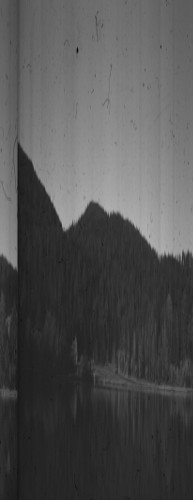
\includegraphics[height=6cm]{images/jpg/extract_image_3.jpg} }}
  \hspace{3em}
  \subfloat[offset too high: 600]{{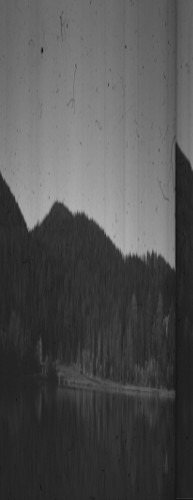
\includegraphics[height=6cm]{images/jpg/extract_image_4.jpg} }}
  \label{extraction_first}
\end{figure}

If the offset is slightly too low, the rightmost part of the image will be moved to the very left.
If it is slightly too high, the leftmost part of the image will be moved to the very right.
An offset of 300 bytes was found to be ideal.

The line offset was adjusted to remove lines not belonging to the main scan, this
can be inspected in an image editor such as GIMP \cite{gimp}. A line offset of 840 was found to
look good, removing unwanted lines on top while keeping all of the main scan.

\begin{figure}[H]
  \caption{Main scan after adjusting \it{byteOffset, byteNth, lineOffset}}
  \centering
  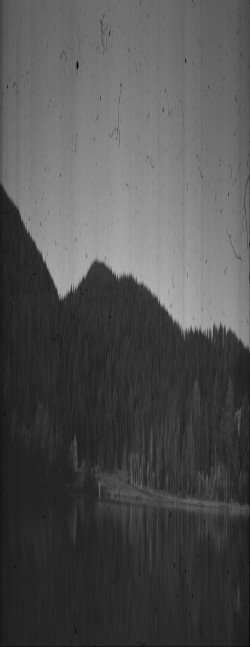
\includegraphics[height=6cm]{images/jpg/extract_image_2.jpg}
  \label{fig:extract_step1}
\end{figure}

\subsubsection{Channel deinterleaving}
\label{ssec:deinterleave}

\begin{figure}[H]
  \caption{Interleaved color channels}
  \centering
  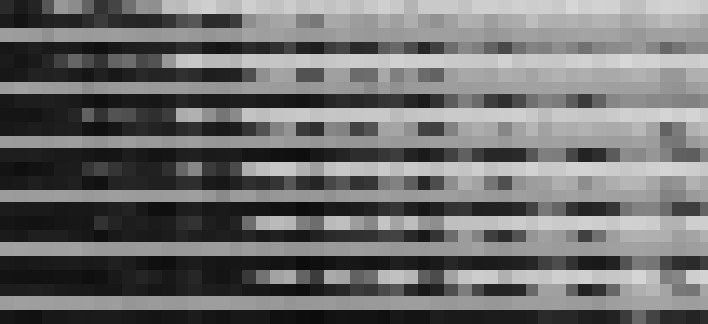
\includegraphics[width=8cm]{images/jpg/extract_image_5.jpg}
\end{figure}

When looking at the image of \autoref{fig:extract_step1} in detail,
the pixels follow an interleaved line pattern of length 4. For each of
the different channels red, green, blue and infrared there is a suitable
value modulo 4 such that the image of this channel is defined by all lines
whose offset is congruent to that value mod 4. This is the purpose of the
{\it --lineNth} option together with a proper {\it --lineOffset}.
{\it --lineNth} is set to 4 and then the previously determined
line offset of 840 is incremented by 0, 1, 2 and 3 to get four separate
color channel images:

\begin{figure}[H]
  \caption{Four different line offsets / color channels}
  \centering
  \subfloat[offset 840]{{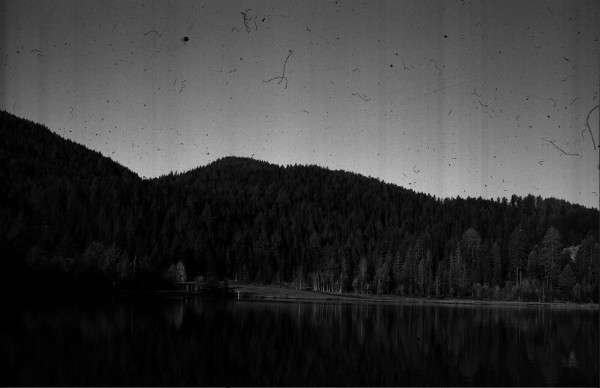
\includegraphics[height=3.5cm]{images/jpg/extract_image_6a.jpg} }} \quad
  \subfloat[offset 841]{{
\includegraphics[height=3.5cm]{images/jpg/extract_image_6b.jpg} }}
  
  \subfloat[offset 842]{{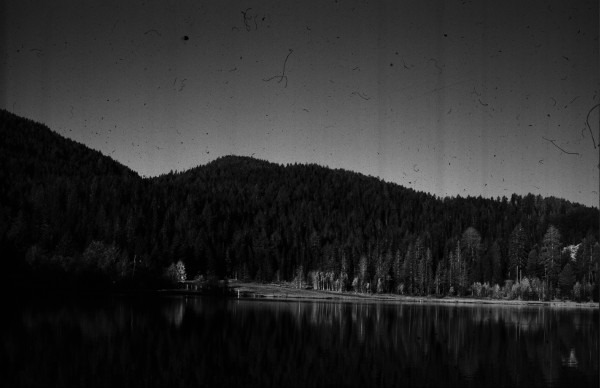
\includegraphics[height=3.5cm]{images/jpg/extract_image_6c.jpg} }} \quad
  \subfloat[offset 843]{{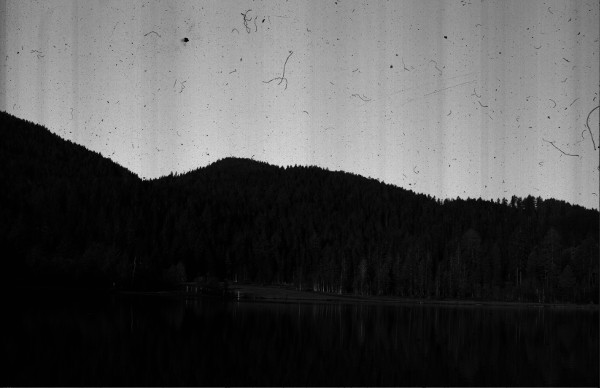
\includegraphics[height=3.5cm]{images/jpg/extract_image_6d.jpg} }}
\end{figure}

Thanks to the choice of image scanned, knowing which offset corresponds to what color channel
is easy: 840 is green, 841 infrared (only dust visible), 842 red (bright yellow trees), 843 blue (bright sky).
The order of channels can vary depending on how much data was skipped at the beginning.

The infrared channel will be used in \autoref{sec:imgproc} to remove dust at the other color channels.

\subsubsection{Channel alignment, combination, gamma correction}
\label{sssec:channelcombine}

The extracted color channels are vertically misaligned, to fix this the
channel which is the furthest "up" (i.e. the channel for which all other channels only need
upwards shifting to align) is determined. Then, for each of the other channels the number
of lines it needs to be moved up to align is determined. This is done visually in GIMP by
opening the channels as layers and reducing the opacity of the channel to be aligned.
The dust specks on the scan are ideal anchors for alignment.

The red channel was found to be the furthest up, the green and infrared channels
needed to be moved up 3 lines and the blue channel 5 lines.
These numbers are multiplied by 4
(because of interleaving) and added to the channel line offsets found in \autoref{ssec:deinterleave}.
The line offsets now are: red 842 (same as before), green 852 (+12), infrared 853 (+12), blue 863 (+20).

Due to the different line offsets, some channels have more lines than others.
For combining channels, all need to be the same size. To achieve this, a maximum
of 1060 lines was kept per channel. This leads to these final parameters:

\begin{table}[H]
  \caption{Final parameters per channel}
  \centering
  \begin{tabular}{l|l|l|l|l|l|l}
    channel & byteOffset & byteNth & lineLength & lineOffset & lineNth & lineMax \\ \hline
    red & 300 & 2 & 1645 & 842 & 4 & 1060 \\
    green & 300 & 2 & 1645 & 852 & 4 & 1060 \\
    blue & 300 & 2 & 1645 & 863 & 4 & 1060 \\
    infrared & 300 & 2 & 1645 & 853 & 4 & 1060 \\
  \end{tabular}
\end{table}

The red, green and blue channels are combined into an RGB image. To make the image look a little
more presentable, a gamma correction with $\gamma = 2$ was applied on each channel.
This means the brightness values get normalized to the range $[0, 1]$,
then a mapping $x \mapsto x^{\frac{1}{2}}$ is applied, then the values are
converted back to the range $[0, 255]$. This is the resulting 1045x1060 color image:

\begin{figure}[H]
  \caption{Extracted image compared to vendor software output}
  \centering
  \subfloat[extracted from capture]{{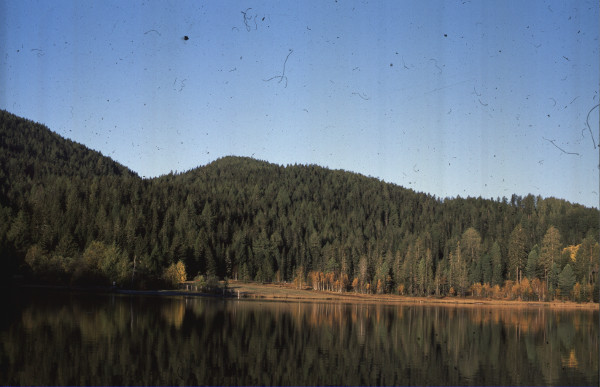
\includegraphics[width=0.6\textwidth]{images/jpg/extract_image_7a.jpg} }}
  
  \subfloat[saved by CyberView X5]{{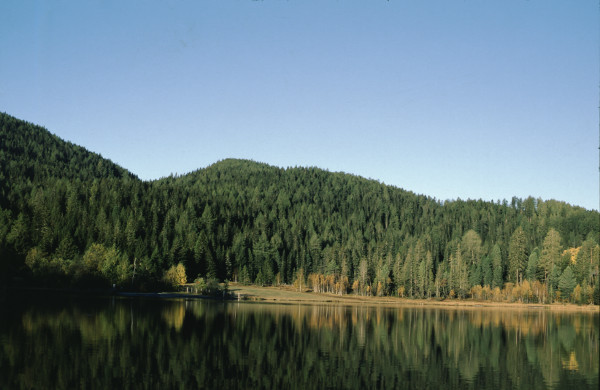
\includegraphics[width=0.6\textwidth]{images/jpg/extract_image_7b.jpg} }}
\end{figure}

The color balance / saturation / contrast is different to the original because of postprocessing
done by CyberView. Vertical stripes on the extracted image could be removed with
the help of the calibration scan.
CyberView also removes dust using the infrared channel (called Digital ICE).

\subsection{Calibration image}
\label{ssec:calibration}

The extracted image has some level of vertical stripes, i.e the brightness is
slightly different per column. This is caused by slight differences in sensitivity
among pixels of the line sensor.
To correct this, the scanner scans a small area where there is only the white background.
This image can be used to "subtract" (actually it's a division operation) the unwanted
brightness differences from the actual scan.
The calibration image is transferred before the other scans: \autoref{ssec:extract_results}

As for the regular scan, we need to identify the right offsets, width, height, and
extract the channels. As these parameters do not vary with scan parameters and the
calibration image covers the whole sensor width, this only
has to be done once. This however means the image needs to be adapted (cropped, downscaled)
based on the vertical area and resolution of the actual scan.

Determining the line width is harder because we don't have a rough guess like the
vendor software image width and there is no image to orient by. It helps that there
is a pattern (darker pixel) at the start of each line. So we can extract the image
with any line size and count the difference in rows and columns between two successive
line starts. We then get the line width by $w_{correct} = (y_b - y_a) \cdot w_{chosen} + x_b - x_a$.
where $y_a, x_a$ are the row and column of the point of the first line start pattern
and $y_b, x_b$ for the second.

\begin{figure}[H]
  \caption{Determining the correct line width for the calibration image (chosen width: 300 pixels)}
  \centering
  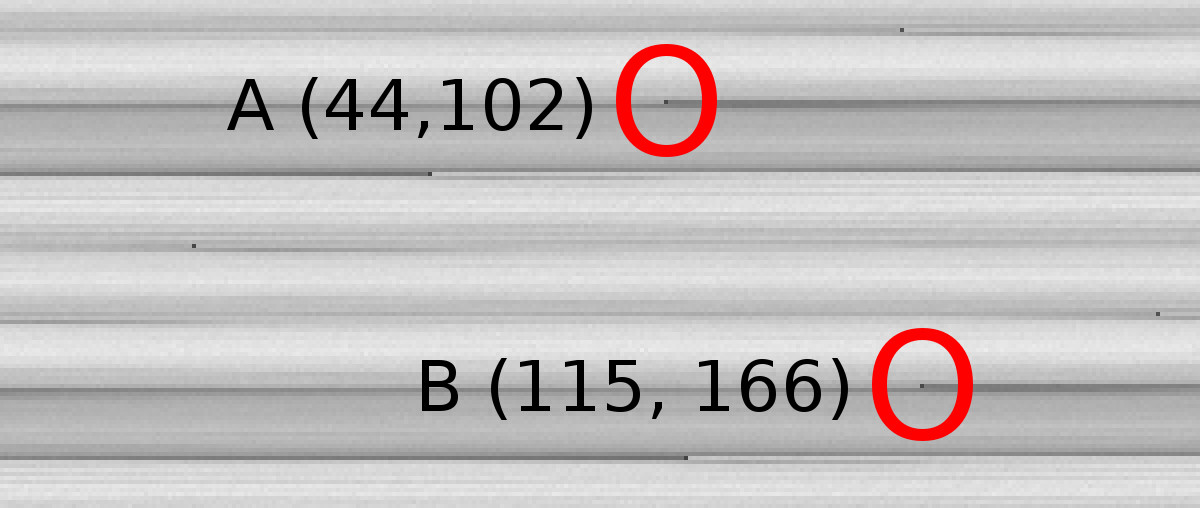
\includegraphics[width=12cm]{images/jpg/extract_calib_1.jpg}
\end{figure}

The correct width was found to be $(115 - 44) \cdot 300 + 166 - 102 = 21364$ pixels.

\begin{figure}[H]
  \caption{Calibration image, width: 21364 pixels}
  \centering
  
\includegraphics[width=12cm, height=2cm]{images/jpg/extract_calib_2.jpg}
\end{figure}

The calibration image has the same channel interleaving pattern as the regular one.
Since we aligned the beginning of a line of some color channel with the next line of that channel,
the 4 channels are side by side.
We extract the different channels by dividing the line width by 4 (5341 pixels)
and using different line offsets.
The final parameters are:

\begin{table}[H]
  \caption{Parameters for the calibration image}
  \centering
  \begin{tabular}{l|l|l|l|l|l|l}
    channel & byteOffset & byteNth & lineLength & lineOffset & lineNth & lineMax \\ \hline
    red & 441 & 2 & 5341 & 0 & 4 & 44 \\
    green & 441 & 2 & 5341 & 1 & 4 & 44 \\
    blue & 441 & 2 & 5341 & 2 & 4 & 44 \\
    infrared & 441 & 2 & 5341 & 3 & 4 & 44 \\
  \end{tabular}
\end{table}


\begin{figure}[H]
  \caption{Calibration images for all four channels}
  \centering
  \subfloat[red]{{
\includegraphics[height=1cm]{images/jpg/extract_calib_3r.jpg} }}
  \subfloat[green]{{
\includegraphics[height=1cm]{images/jpg/extract_calib_3g.jpg} }}
  
  \subfloat[blue]{{
\includegraphics[height=1cm]{images/jpg/extract_calib_3b.jpg} }}
  \subfloat[infrared]{{
\includegraphics[height=1cm]{images/jpg/extract_calib_3i.jpg} }}
\end{figure}

Applying the calibration image to the actual scan is shown in \autoref{ssec:imgproc_calib}.

\section{Controlling the device}

\subsection{Setup: PyUSB}

PyUSB \cite{pyusb} is a Python module for accessing USB devices.
Using it is straightforward:
A handle for the device is created by specifying the characteristic
vendor and product ID (these are for my scanner, can be found via {\it lsusb}):

\begin{center}
\tt dev = usb.core.find(idVendor=0x05e3, idProduct=0x0145)
\end{center}

After finding the scanner, like any USB device it needs to be configured
before using it. This means choosing one of the available configuration
profiles (described by configuration descriptors). The scanner, like most
devices, only has one configuration. It can be selected with:

\begin{center}
\tt dev.set\_configuration(0)
\end{center}

After configuring the device, control and bulk transfers can be initiated.
Control transfers are initiated like this:

\begin{center}
\tt
dev.ctrl\_transfer(self, bmRequestType, bRequest, wValue, wIndex, data\_or\_wLength, timeout)
\end{center}

{\it bmRequestType, bRequest, wValue, wIndex, wLength} are described in \autoref{table:ctrltransfer}.
timeout specifies the number of milliseconds after which the transfer is canceled if
still not completed.

For host-to-device control transfers, {\it data\_or\_wLength} contains the data payload
and the return value is the number of bytes actually written. The wLength parameter
is inferred from the length of the payload bytestring.

For device-to-host control transfers, {\it data\_or\_wLength} contains the wLength
parameter specifying the number of bytes to be read and the return value is the payload
received from the device.

As opposed to control transfers, bulk transfers have no structure at the layer
of the USB standard and can be imagined as reading from / writing to a byte stream.
They are self-explanatory:

\begin{center}
\tt
dev.read(endpoint, size, timeout)

dev.write(endpoint, data, timeout)
\end{center}

PyUSB was used to create a simple scanning program {\it scanInteractive.py}
which performs a scan with certain parameters, does basic image processing
(see \autoref{sec:extract}) and displays the image building up row by row
as data is received from the scanner.

\subsection{Vendor-specific control transfers}

USB traffic starts when the scanner software loads and continues
constantly while the software is running (even when idling).
It consists of vendor-specific control transfers on endpoint 0
in both directions: bmRequestType 0x40 outgoing / 0xc0 incoming, see \autoref{table:ctrltransfer}.
Also there are incoming bulk transfers on endpoint 1, used both for
receiving status information and image data.

These combinations of control transfer parameters were observed
while the software was idling / scanning:

\begin{table}[H]
  \caption{Control transfer parameter combinations}
  \centering
  \begin{tabular}{l|l|l|l|l|l}
    Combination & bmRequestType & bRequest & wValue & wIndex & wLength \\ \hline
    a) & 0x40 (outgoing) & 4 & 0x0082 & 0 & 8 \\
    b) & 0xc0 (incoming) & 12 & 0x0084 & 0 & 1 \\
    c) & 0x40 (outgoing) & 12 & 0x0085 & 0 & 1 \\
    d) & 0x40 (outgoing) & 12 & 0x0087 & 0 & 1 \\
    e) & 0x40 (outgoing) & 12 & 0x0088 & 0 & 1 \\
  \end{tabular}
  \label{table:paramcombos}
\end{table}

These additional parameter combinations were only observed during software
startup:

\begin{table}[H]
  \caption{Parameter combinations at startup}
  \centering
  \begin{tabular}{l|l|l|l|l|l}
    Combination & bmRequestType & bRequest & wValue & wIndex & wLength \\ \hline
    f) & 0x40 (outgoing) & 12 & 0x0089 & 0xf49c & 1 \\
    g) & 0xc0 (incoming) & 12 & 0x008a & 0x008b & 1 \\
    h) & 0x40 (outgoing) & 12 & 0x008b & varies & 1 \\
    i) & 0x40 (outgoing) & 12 & 0x008c & 0x0010 & 1 \\
    j) & 0xc0 (incoming) & 12 & 0x008e & 0 & 1 \\
  \end{tabular}
\end{table}

In addition to the parameters, control transfers have a data payload that is {\it wLength} bytes long \autoref{table:ctrltransfer}.
The actual commands regarding what the device should do are encoded in this data payload.
As all but one parameter combination has a one-byte payload, most commands are transferred
one byte after another, doing one control transfer for each byte.

\subsection{Transaction patterns}
\label{ssec:transactionpatterns}

All traffic during idling and scanning can be modeled by transactions: Each transaction
starts with the same header. After that, six parameter bytes are sent and the
device response is queried. The rest depends on the transaction type, there
are four types of transaction: The most basic does not do anything besides sending parameters and querying the response.
One kind of transaction transmits additional parameter bytes, another reads more detailed device status
and the fourth kind is used for retrieving image data.

\subsubsection{Header}

Every transaction begins with the same header that consists of these 11 control transfers:

\begin{table}[H]
  \caption{Header structure for all three transaction types}
  \centering
  \begin{tabular}{l|l|l}
    Nr. & Parameters \autoref{table:paramcombos} & Data payload \\ \hline
    1. & e) & 0xff \\
    2. & e) & 0xaa \\
    3. & e) & 0x55 \\
    4. & e) & 0x00 \\
    5. & e) & 0xff \\
    6. & e) & 0x87 \\
    7. & e) & 0x78 \\
    8. & e) & 0xe0 \\
    9. & d) & 0x05 \\
    10. & d) & 0x04 \\
    11. & e) & 0xff \\
  \end{tabular}
  \label{table:transheader}
\end{table}

\subsection{Device readiness query}
\label{ssec:devready}

At the end of each transaction, but also at other points (like before
sending extra parameters, before transferring image data) the software has to ask for a device response.

This is done using a control transfer with parameter combination b) in \autoref{table:paramcombos}.

\begin{table}[H]
  \caption{Device readiness responses}
  \centering
  \begin{tabularx}{\textwidth}{l | X}
    Response & Meaning \\ \hline
    {\tt 0x00} & OK, returned inside extra parameter transaction (before sending extra parameters) \\
    {\tt 0x01} & OK, returned in status / image transaction, before doing bulk reads \\
    {\tt 0x03} & Read another response byte, see \autoref{table:devready_2} \\
  \end{tabularx}
\end{table}

When the first response byte is {\tt 0x03}, the control transfer needs to be repeated for another
response byte. Such a two-byte response means the transaction is now complete (if in the middle
of an image / status transaction, do not continue with this transaction, but repeat the transaction from the start).

\begin{table}[H]
  \caption{Second response byte}
  \centering
  \begin{tabularx}{\textwidth}{l | X}
    Response & Meaning \\ \hline
    {\tt 0x00} & OK. Continue with next transaction. \\
    {\tt 0x02} & Failure due to wrong commands sent by software. Should not happen during normal operation. \\
    {\tt 0x08} & Device not ready yet. Repeat transaction. \\
  \end{tabularx}
  \label{table:devready_2}
\end{table}

\subsection{Reading from the bulk endpoint}
\label{ssec:bulkread}

For a status transaction or image transaction, data needs to be read from the bulk endpoint of the device.
This has to be done using a special pattern:

First, a control transfer (combination a) in \autoref{table:paramcombos}) is
performed with the following 8-byte payload (hex): {\tt 00000000xxyy0000},
where the number of bytes to be read ($c$, $1 \leq c \leq 65520$) from the bulk endpoint is encoded
in little-endian format, i.e. bytes at offset 4 and 5 ({\tt xx} and {\tt yy}) are set such that
$c = 256 * \texttt{yy} + \texttt{xx}$.

Then the actual bulk read transfer of $c$ bytes from endpoint 1 can happen. The vendor software
splits large transfers into multiple smaller transfers, but this does not seem
to be necessary.

\subsection{Basic transaction}
\label{ssec:basic_trans}

This type of transaction has the simplest structure. It is used only for a handful of tasks like
checking device readiness at critical points and the actual "start scan" command.
Details about the transaction parameters can be found in \autoref{appendix_basic}.

\subsubsection{Structure}

\begin{table}[H]
  \caption{Structure of the basic transaction}
  \centering
  \begin{tabularx}{\textwidth}{X | X | X | X}
    Stage & No. of transfers / bytes & Transfer parameters & Data payload \\ \hline
    
    Header & 11 & see \autoref{table:transheader} & see \autoref{table:transheader} \\
    Main parameters & 6 & c) in \autoref{table:paramcombos} & see \autoref{appendix_basic} \\
    Device response & 2 & b) in \autoref{table:paramcombos} & see \autoref{ssec:devready} \\
  \end{tabularx}
\end{table}


\subsection{Extra parameter transaction}

This transaction is used to set parameters while preparing a scan.
The bytestring of the "Main parameter" stage defines the purpose of the transaction
(e.g. setting resolution / exposure parameters). The "Extra parameter" stage
transfers the values of the parameters that should be set.
Details about the transaction parameters can be found in \autoref{appendix_extra}.

\subsubsection{Structure}

\begin{table}[H]
  \caption{Structure of the extra parameter transaction}
  \centering
  \begin{tabularx}{\textwidth}{X|X|X|X}
    Stage & No. of transfers / bytes & Transfer parameters & Data payload \\ \hline
    
    Header & 11 & see \autoref{table:transheader} & see \autoref{table:transheader} \\
    Main parameters & 6 & c) in \autoref{table:paramcombos} & see \autoref{appendix_extra} \\
    Device response & 1 & b) in \autoref{table:paramcombos} & see \autoref{ssec:devready}, {\tt 0x00} expected \\
    Extra parameters & varies, see \autoref{appendix_extra} & c) in \autoref{table:paramcombos} & see \autoref{appendix_extra} \\
    Device response & 2 & b) in \autoref{table:paramcombos} & see \autoref{ssec:devready} \\
  \end{tabularx}
\end{table}

\subsection{Status transaction}
\label{ssec:read_trans}

This is used to read device status from the bulk endpoint.
Details about the transaction parameters can be found in \autoref{appendix_status}.

\subsubsection{Structure}

\begin{table}[H]
  \caption{Structure of the read transaction}
  \centering
  \begin{tabularx}{\textwidth}{X|X|X|X}
    Stage & No. of transfers / bytes & Transfer parameters & Data payload \\ \hline
    
    Header & 11 & see \autoref{table:transheader} & see \autoref{table:transheader} \\
    Main parameters & 6 & c) in \autoref{table:paramcombos} & see \autoref{appendix_status} \\
    Device response & 1 & b) in \autoref{table:paramcombos} & see \autoref{ssec:devready}, {\tt 0x01} expected \\
    Bulk read & see \autoref{appendix_status} & see \autoref{ssec:bulkread} & see \autoref{ssec:bulkread} \\
    Device response & 2 & b) in \autoref{table:paramcombos} & see \autoref{ssec:devready} \\
  \end{tabularx}
\end{table}


\subsection{Image transaction}

The image transaction is used for receiving the calibration and the main image.

\subsubsection{Structure}

\begin{table}[H]
  \caption{Structure of the image transaction}
  \centering
  \begin{tabularx}{\textwidth}{X|X|X|X}
    Stage & No. of transfers / bytes & Transfer parameters & Data payload \\ \hline
    
    Header & 11 & see \autoref{table:transheader} & see \autoref{table:transheader} \\
    Main parameters & 6 & c) in \autoref{table:paramcombos} & see \autoref{ssec:image_param} \\
    Device response & 1 & b) in \autoref{table:paramcombos} & see \autoref{ssec:devready} \\
    Bulk reads & see \autoref{ssec:image_bulk} & see \autoref{ssec:bulkread} & see \autoref{ssec:bulkread} \\
    Device response & 2 & b) in \autoref{table:paramcombos} & see \autoref{ssec:devready} \\
  \end{tabularx}
\end{table}

\subsubsection{Main parameters}
\label{ssec:image_param}

An image transaction has the parameter string (hex) {\tt 08000000xx00}.
The byte at offset 4 represents the number of lines of the image that
should be received.
g
An image transaction that transfers for example 14 lines would be identical
up to the main parameter stage
to an extra parameter transaction with main parameter string {\tt 080000000e00}.
The device response after the main parameter stage however has to be different
(0x00 for extra parameter, 0x01 for image). This shows that the device has
to consider context when analyzing the meaning of a transaction's main parameters
({\tt 080000000e00} means "set scan area" while preparing the scan but
"transfer 14 lines" after the scan has started).

\blockquote[{\cite[\tt pieusb\_scancmd.c, sanei\_pieusb\_cmd\_start\_scan()]{sane_code}}]
{This is a SCSI READ command (code 0x08).
 It is distinguished from the other READ commands by the context
 in which it is issued. \\}

\subsubsection{Bulk reads}
\label{ssec:image_bulk}

In this stage, the image data is transferred using one ore more
bulk reads (see \autoref{ssec:bulkread}).

For this, the amount of bytes per line of the image $c_l$ needs to be known
(see \autoref{table:imageparam_query}). This is multiplied by the number of lines $l$ to be transferred
to get the total amount of bytes to be transferred:

\begin{center}
\begin{tabular}{l}
$ c = c_l * l $
\end{tabular}
\end{center}

This amount gets divided into 65520 ({\tt 0xfff0}) byte chunks plus a possible rest:

\begin{center}
\begin{tabular}{l}
$n = \lfloor \frac{c}{65520} \rfloor $ \\
$m = c \mod 65520$ \\
\end{tabular}
\end{center}

The data is transferred in $n$ 65520-byte reads followed by one $m$-byte
read (if m is nonzero).

\subsection{Receiving the calibration image}
\label{ssec:rcv_calibimage}

The size and format of the calibration image does not depend on the scanner settings.
On this scanner, it has 180 (45 per channel) lines of 5341 16-bit pixels (10682 bytes).
The total calibration image size is 1922760 bytes.

The lines follow a RGBI channel interleaving (see \autoref{sec:extract}).

In the actual scan (\autoref{ssec:actualscan}), at first 4 lines get transferred, then 172, then the last 4.

\subsection{Receiving the main image}
\label{ssec:rcv_mainimage}

When receiving the main image, it is essential to know how many lines the image
has and how many bytes there are per line. These values are used to generate image transactions.

The number of lines $l$ gets divided into 255-line chunks plus a possible rest:

\begin{center}
\begin{tabular}{l}
$n = \lfloor \frac{c}{255} \rfloor $ \\
$m = c \mod 255$ \\
\end{tabular}
\end{center}

The image is transferred in $n$ 255-line image transactions followed by one $m$-line
image transaction (if m is nonzero). Each mage transactions itself of course needs
to be adjusted to its line count and the number of bytes per line.

If the data is read faster than the scanner can produce it, the device readiness
response in the middle of the image transaction will return a busy status. In this case,
just repeat this image transaction until the scanner is ready.

\subsection{Timing}

Suppose you have a recording of all USB traffic that happened during a scan.
It would not be sufficient to just replay all the recorded outgoing packets
at once (and wait for incoming packets at the right points).

This is due to the importance of timing. At certain points, the device
is not immediately ready for the next command. The most important point
where this is the case is after starting the scan before doing the first
image transaction. To ensure device readiness, a basic query (\autoref{ssec:basic_trans})
is used. The device response (\autoref{ssec:devready}) in this query returns "busy" if the device
is not ready yet. After receiving a busy response, the software should sleep
for a bit (the vendor software uses a 1.5 second interval) and repeat the basic transaction
until the device responds that it's not busy.

Something similar happens when doing image transactions faster than the device
can scan the lines. Before the bulk read stage, the device responds "busy"
and the image transaction should be repeated from the start (\autoref{ssec:rcv_mainimage}).

\begin{figure}[H]
  \caption{Timing of packets during scan}
  \centering
  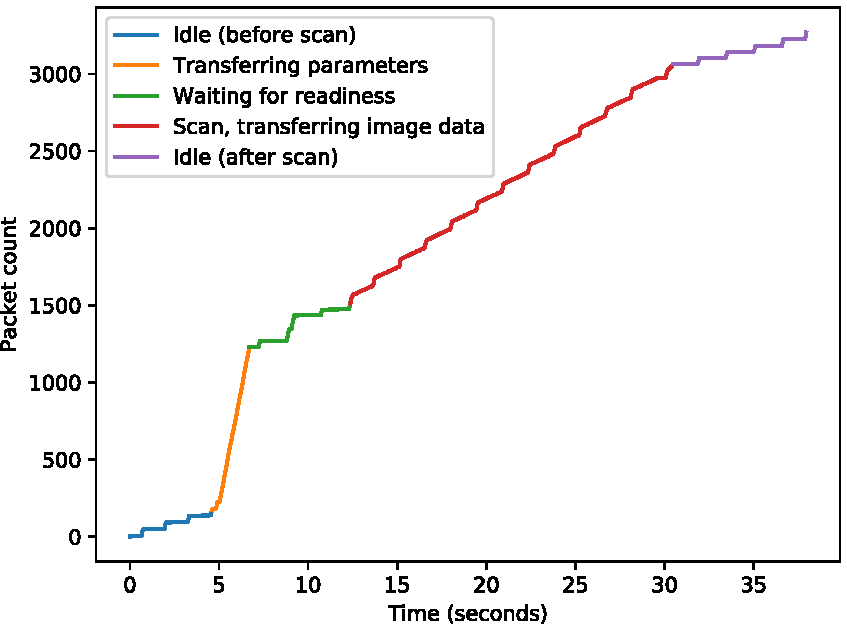
\includegraphics[width=\textwidth]{images/pdf/time_diagram_eng.pdf}
  \label{time_diagram}
\end{figure}

This diagram illustrates the rate at which packets are transmitted
during a simple scan (no prescan, no calibration) with the vendor-supplied
(CyberView X5) software.
The scanning process can be separated into five phases:

\begin{enumerate}

\item During the idle phase before the scan, every 1.5 seconds a status read query
(\autoref{ssec:read_trans}) is performed.

\item When the user presses "start scan", all scan parameters being transferred
in rapid succession causes a quick increase in packet count.

\item After the parameters are sent to the device, but before the image is transferred
the software has to wait for readiness (1.5 second waits in between a basic transaction
which shows as a burst of packets).

\item During the image transaction stage, each image transaction's header is
transferred quickly. The transfer of the actual image lines happens without waits
but more slowly (the curve climbs diagonally) due to the large amount of data.

\item After the scan has completed and the image is fully transferred,
the traffic returns to the idle pattern again. Interestingly, the delay
between status queries is now slightly longer (about 2s) than before the scan.

\end{enumerate}

\subsection{An actual scan}
\label{ssec:actualscan}

All the USB traffic that happens during an actual scan can be represented
using the transaction patterns described in this section. To better illustrate
how an actual scan proceeds, an example using a list of transactions is described.

A prescan (includes receiving calibration image) was selected in the vendor software
for its calibration image but also because its transactions can be replayed
to the device straight after the scanner has started
(not possible with a regular scan, the device needs to do at least one pre-scan
after having started).

The scan parameters and USB traffic (modeled in these transactions) can be found
in \autoref{appendix_actualscan}.

\section{SANE}
\label{sec:sane}

SANE (abbreviated for "Scanner Access Now Easy") is the standard software package
for accessing scanners in Linux-like operating systems. SANE was created
because previous scanner software packages were often specific to a single device / vendor.
Its most notable feature is the separation between backend (device driver) 
and frontend (user scanning software).

SANE contains many different backends for devices of different manufacturers.
A lot of these drivers were not provided by manufacturers but instead
developed by hobbyists using various reverse-engineering procedures.

Another unique feature is {\it saned}, which is a server daemon that allows
scanning over a network. This is desirable since one can share a scanner
among multiple machines in the same location. When using {\it saned}, a
special {\it net} backend is used on the client machine to make
the remote scanner accessible just like a local one in the user's preferred frontend.

SANE frontends include {\it scanimage} for scanning on the command line,
{\it xsane} for a graphical interface and a web application that can be served
on a network and accessed via web browser, this is another way of providing shared
scanner access.

\begin{figure}[H]
  \caption{Example SANE hierarchy (after \cite[Figure 3.1]{sane_standard})}
  \centering
  \resizebox{\textwidth}{!}{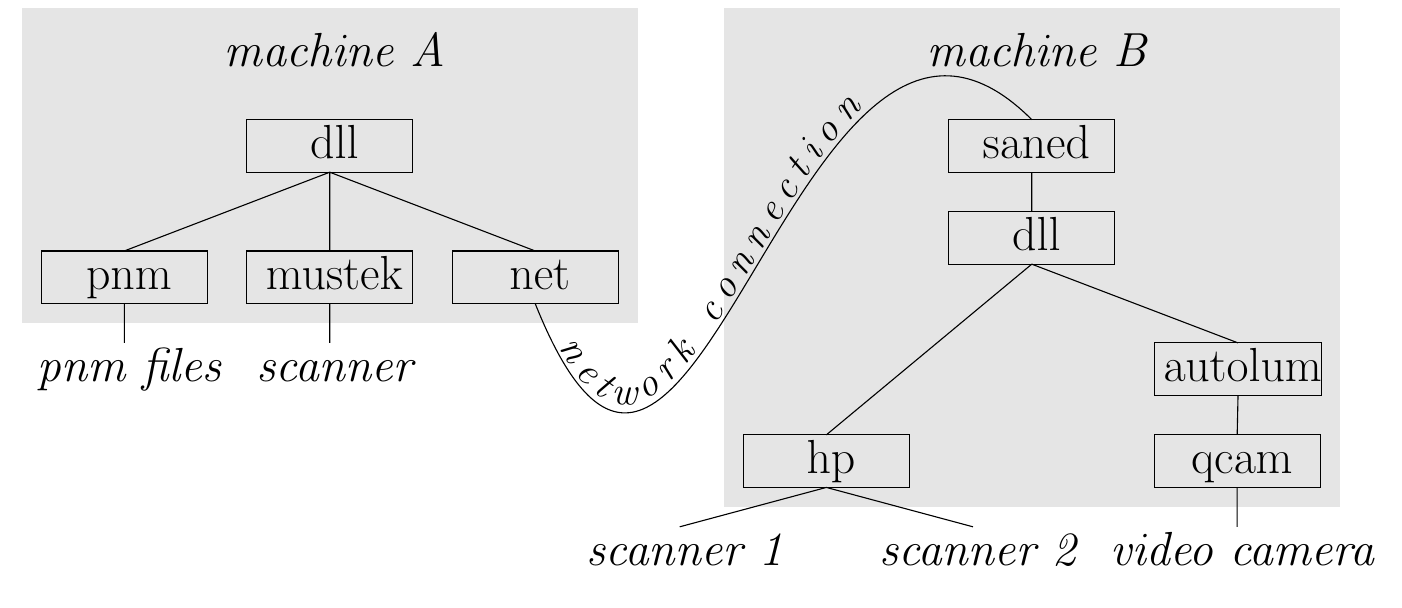
\begin{tikzpicture}
\pgfdeclarelayer{background}
\pgfsetlayers{background,main}

\tikzset{font={\fontsize{16}{16} \selectfont}}

\tikzset{nstyle/.style={
  inner sep=0,
  outer sep=0,
  text height=14,
  text depth=5,
  minimum width=60,
}}

\node[style=nstyle] (machineA) {\it machine A};
\node[style=nstyle, draw, below = 0.5 of machineA] (dll) {dll};
\node[style=nstyle, draw, below = 1 of dll] (mustek) {mustek};
\node[style=nstyle, draw, left = 0.5 of mustek] (pnm) {pnm};
\node[style=nstyle, draw, right = 0.5 of mustek] (net) {net};
\node[style=nstyle, below = 0.5 of pnm] (pnmFiles) {\it pnm files};
\node[style=nstyle, below = 0.5 of mustek] (scanner) {\it scanner};

\node[style=nstyle, right = 6 of machineA] (machineB) {\it machine B};
\node[style=nstyle, draw, below = 0.5 of machineB] (saned) {saned};
\node[style=nstyle, draw, below = 0.5 of saned] (dll2) {dll};
\node[style=nstyle, below = 1 of dll2] (hidden1) {};
\node[style=nstyle, below = 0.5 of hidden1] (hidden2) {};
\node[style=nstyle, draw, right = 0.5 of hidden1] (autolum) {autolum};
\node[style=nstyle, draw, right = 0.5 of hidden2] (qcam) {qcam};
\node[style=nstyle, draw, left = 0.5 of hidden2] (hp) {hp};
\node[style=nstyle, below left = 0.5 and -0.5 of hp] (scanner1) {\it scanner 1};
\node[style=nstyle, below right = 0.5 and -0.5 of hp] (scanner2) {\it scanner 2};
\node[style=nstyle, below = 0.5 of qcam] (camera) {\it video camera};

\draw
  (dll.south) -- (mustek.north)
  (dll.south) -- (pnm.north)
  (dll.south) -- (net.north)
  (pnm.south) -- (pnmFiles.north)
  (mustek.south) -- (scanner.north)
  (saned.south) -- (dll2.north)
  (dll2.south) -- (autolum.north)
  (autolum.south) -- (qcam.north)
  (dll2.south) -- (hp.north)
  (hp.south) -- (scanner1.north)
  (hp.south) -- (scanner2.north)
  (qcam.south) -- (camera.north);

\useasboundingbox (0,0) rectangle (0,0);

\draw
  (net.south)
  .. controls ($(net.south) + (2, -5)$) and
              ($(saned.north) + (-3, 3)$)
  .. (saned.north);

\path [postaction={decorate, 
       decoration={text along path,
                   text align={left,
                               left indent=20pt,
                               right indent=70pt,
                               fit to path},
                   text={|\it \Large|network connection}}}]
  ($(net.south) + (0, 0.1)$)
  .. controls ($(net.south) + (2, -5) + (0, 0.1)$) and
              ($(saned.north) + (-3, 3) + (0, 0.1)$)
  .. ($(saned.north) + (0, 0.1)$);

\begin{pgfonlayer}{background}
  \fill[gray!20] ($(pnm.north west)!(machineA.north west)!(pnm.south west) + (-0.25,0.25)$)
    rectangle ($(net.south east) + (0.25,-0.25)$);
  \fill[gray!20] ($(hp.north west)!(machineB.north west)!(hp.south west) + (-0.25,0.25)$)
    rectangle ($(qcam.south east) + (0.25,-0.25)$);
\end{pgfonlayer}


\end{tikzpicture}
}
  \label{sane_hierarchy}
\end{figure}

\subsection{The SANE standard}
\label{ssec:sanestd}

As mentioned before, SANE consists of backends (that manage devices) and frontends
(that provide applications). Any backend can be combined with any frontend
thanks to the SANE interface / standard. In theory there could be multiple independent
implementations of this standard, however only the official SANE package is
commonly used.

The SANE interface is an application programming interface (API) consisting
of specified C procedures / types that are implemented by backends and called by frontends.
Frontend and backend can be combined either by static or dynamic linking.
To make a frontend support multiple backends, the frontend can be linked to a
meta-backend that finds out which backend is suitable for the currently attached
scanner, loads it via dynamic linking, and then mimics the behavior
of the suitable backend. \cite[3.1]{sane_standard}

\subsubsection{Primitive types}

The standard defines various primitive data types
({\it SANE\_Bool, SANE\_Byte, SANE\_Word, SANE\_Fixed, SANE\_String})
which have certain guaranteed qualities
like minimum number of bytes, endianness etc. to mitigate differences in
C compilers and hardware.

There is also an enum type {\it SANE\_Status} which operations use to report back on
status.

\subsubsection{Device descriptor}

The device descriptor contains identifying information about a scanner (name / model),
is returned by the {\it sane\_get\_devices} procedure and is used to obtain a device handle
from the {\it sane\_open} procedure.

\subsubsection{Scanner handle}

The scanner handle is a pointer that is returned by {\it sane\_open} and is used to
control the scanner using SANE operations (get / set options, start scan).

\subsubsection{Options}

Options are a powerful feature of the SANE standard in that the same type and procedures
are used to control every setting on a device: basic ones like resolution or scan area, but also
device-specific settings; this is independent of manufacturer / backend.

The option descriptor is a struct type with various components specifying an option's
meaning and its possible values: name (unique identifier),
title (human-readable name), description, type (bool / string etc.), unit (pixels / millimeters etc.)
and constraints (f.e. a range of possible coordinate values in a dimension,
a list of allowed string values). \cite[4.2.9]{sane_standard}

Every device handle has a certain number of option descriptors associated
with it. An option descriptor can be fetched with the {\it sane\_get\_option\_descriptor}
procedure by specifying the index of the option.
Backends can define any number of custom option descriptors, but some
descriptors' meaning is specified in the standard:

\begin{table}[H]
  \caption{Special option descriptors specified in the SANE standard \cite[4.5]{sane_standard}}
  \centering
  \begin{tabularx}{\textwidth}{l | X}
    Name & Description \\ \hline
      Option count & Always available at index 0. Tells how many options
                            there are in total. \\
      {\it resolution} & Scan resolution (in dpi) \\
      {\it preview} & Bool type, trade scan quality for speed when enabled \\
      Scan area & Four options ({\it tl-x, tl-y, br-x, br-y}) that give
                  the coordinates of a rectangle delimiting the scan area. \\
  \end{tabularx}
\end{table} 

Options values are queried/set using the {\it sane\_control\_option} procedure
specifying the option index and a generic pointer to load / store the value.
This also reports back on how well the request could be met (f.e. a resolution could
not be set exactly) and whether the changed setting has changed the availability
of other options. \cite[4.4]{sane_standard}

\subsubsection{Operations}

The standard specifies various procedures for initialization, configuring options,
scanning and retrieving data.

\begin{table}[H]
  \caption{Operations defined in the SANE standard (not exhaustive) \cite[4.3]{sane_standard}}
  \centering
  \begin{tabularx}{\textwidth}{l | X}
    Name & Description \\ \hline
    \it sane\_init & Must be called before using other procedures of the backend \\
    \it sane\_get\_devices & Get a list of device descriptors, one for each device
                             the backend has found. \\
    \it sane\_open & Initialize the device with a specified descriptor. Returns \\
    \it sane\_close & Free scanner handle \\
    \it sane\_exit & Free data in backend \\
    \it sane\_get\_option\_descriptor & Get the option descriptor at the specified index. \\
    \it sane\_control\_option & Set or retrieve an option value at the specified option index. \\
    \it sane\_get\_parameters & Get parameters (format / dimensions) of image returned by {\it sane\_read}. \\
    \it sane\_start & Start scanning \\
    \it sane\_read & Read retrieved image bytes \\
    \it sane\_cancel & Cancel a scan in progress \\
  \end{tabularx}
\end{table}

When using SANE, typical code flow might look as follows:

\begin{figure}[H]
  \caption{Typical code flow when using SANE \cite[4.4]{sane_standard}}
  \centering
  \scalebox{1}{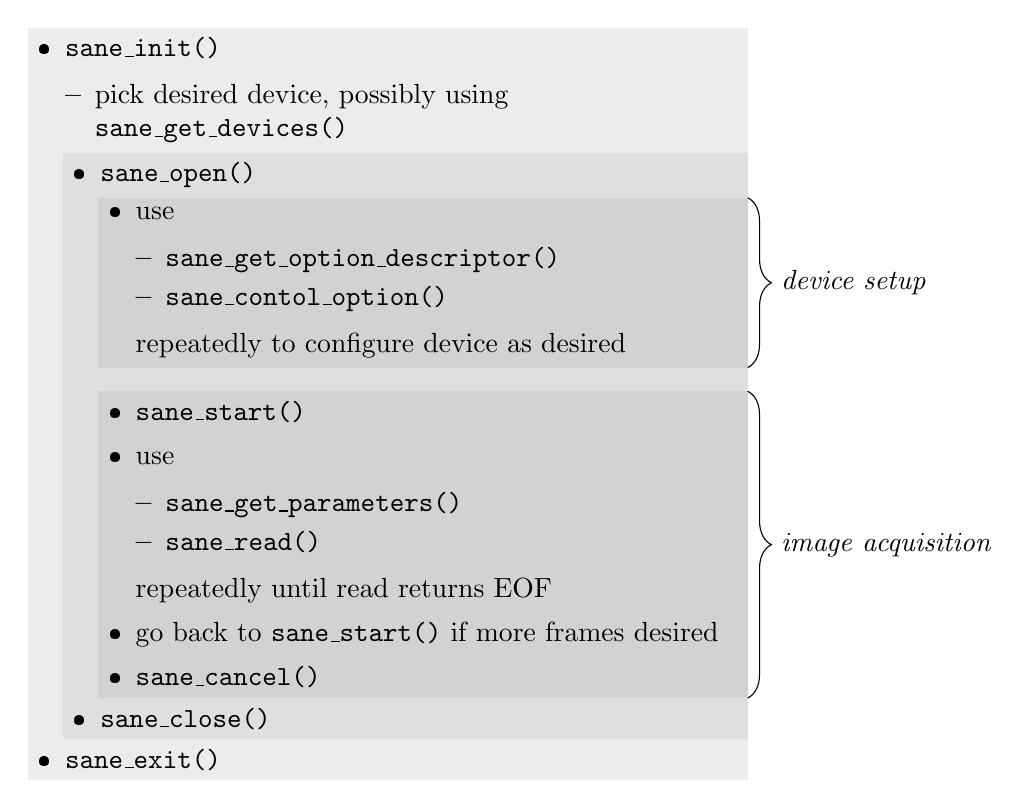
\begin{tikzpicture}
\pgfdeclarelayer{background}
\pgfsetlayers{background,main}
\setitemize{leftmargin=*,topsep=5pt,partopsep=0pt,parsep=0pt}
\node (A) { \begin{minipage}{8cm}
  \begin{itemize}
    \item {\tt sane\_init()}
      \begin{itemize}
      \item pick desired device, possibly using \\{\tt sane\_get\_devices()}
      \end{itemize}
  \end{itemize}
  \end{minipage}
};

\node[below right = 0 and -7.8 of A] (B) { \begin{minipage}{8cm}
  \begin{itemize}
    \item {\tt sane\_open()}
  \end{itemize}
  \end{minipage}
};

\node[below right = 0 and -7.8 of B] (C) { \begin{minipage}{8cm}
  \begin{itemize}
    \item use
      \begin{itemize}
        \item {\tt sane\_get\_option\_descriptor()}
        \item {\tt sane\_contol\_option()}
      \end{itemize}
      repeatedly to configure device as desired
  \end{itemize}
  \end{minipage}
};
\node[below = 0.3 of C] (D) { \begin{minipage}{8cm}
  \begin{itemize}
    \item {\tt sane\_start()}
    \item use
      \begin{itemize}
        \item {\tt sane\_get\_parameters()}
        \item {\tt sane\_read()}
      \end{itemize}
      repeatedly until read returns EOF
    \item go back to {\tt sane\_start()} if more frames desired
    \item {\tt sane\_cancel()}
  \end{itemize}
  \end{minipage}
};

\node[below left = 0 and -7.8 of D] (E) { \begin{minipage}{8cm}
  \begin{itemize}
    \item {\tt sane\_close()}
  \end{itemize}
  \end{minipage}
};

\node[below left = 0 and -7.8 of E] (F) { \begin{minipage}{8cm}
  \begin{itemize}
    \item {\tt sane\_exit()}
  \end{itemize}
  \end{minipage}
};

\draw[decorate, decoration={brace, amplitude=3mm}]
  (C.north east) -- (C.south east)
  node[midway,right=0.3] {\it device setup};

\draw[decorate, decoration={brace, amplitude=3mm}]
  (D.north east) -- (D.south east)
  node[midway,right=0.3] {\it image acquisition};
\begin{pgfonlayer}{background}
  \fill[gray!15] (A.north west) rectangle ($(D.north east)!(F.south east)!(D.south east)$);
  \fill[gray!25] (B.north west) rectangle ($(D.north east)!(E.south east)!(D.south east)$);
  \fill[gray!35] (C.north west) rectangle (C.south east);
  \fill[gray!35] (D.north west) rectangle (D.south east);
\end{pgfonlayer}
\end{tikzpicture}
}
  \label{sane_codeflow}
\end{figure}

\subsubsection{Network protocol}

This specifies how a SANE daemon should communicate with a client, possibly on a
remote machine. This protocol is done in a RPC (remote-procedure-call) style:
The client calls procedures on the server in a similar fashion to how they are
called locally: The parameters are encoded in a packet, sent over the network,
unpacked at the server, the procedure is executed there, the return value takes
the reverse direction.

The exact encoding of packets is not specified (TCP/IP is not the only possible
transport layer), for compatibility it seems reasonable to consider the official
implementations of {\it saned} ( server) and the {\it net} backend (client). \cite[5]{sane_standard}

\subsection{Developing a driver / backend}

The SANE developers give some tips on writing a backend \cite{sane_develop}:

\begin{itemize}
  \item First, one should acquire information on how the device is controlled. This
        can be official documentation released by the manufacturer or obtained via
        various kinds of reverse engineering (software, firmware, sniffing, hardware...).
  \item It is advisable to first write a minimal, working standalone scanning program not part of SANE.
        This makes debugging easier.
  \item After the standalone program is working, one can start developing the backend:
        If the standalone program is already written in C, its code can be copied
        into the backend files and called by the public backend procedures.
\end{itemize}

\cite{sane_develop_re} is focused on reverse-engineering
Windows-only scanners for SANE. Despite being somewhat outdated and referring mostly
to older SCSI scanners, the website provides useful information:

\begin{itemize}
  \item As an alternative to sniffing, Windows drivers could be disassembled
        using special toolkits
  \item There is sniffing software running inside Windows (as an alternative to
        the Linux-based sniffing used here)
  \item Write down information about every scan run performed to keep track which
        settings give which recording
  \item Change only one option per scan run so the changes in traffic can be correlated
        with that option
  \item Keep scan area small to reduce recording size
  \item Constant bursts of traffic while idling may indicate polling for a pressed "start
        scan" button on the device
  \item Modern USB scanners have two levels of communication: One is how to set parameter
        strings and another is the meaning of the bytes inside the parameter string.
        Try to understand the first level first.
  \item If large chunks of data are transmitted, think about their meaning:
        What the driver sends could be firmware code, calibration data, 
        motor acceleration data, gamma tables. The device could send calibration data or actual image data.
\end{itemize}

\subsection{SANE and the CrystalScan 7200}

\subsubsection{pieusb}

{\it pieusb} is a SANE backend that supports the CrystalScan 7200 among
other scanners sold under the Reflecta brand. Development began
in 2012 by Klaus Kaempf et al., in 2015 it got merged into mainline SANE code.
Supported devices include:

\begin{itemize}
  \item Reflecta CrystalScan 7200
  \item Reflecta ProScan 7200
  \item Reflecta 6000 Multiple Slide Scanner
\end{itemize}

The version of SANE / {\it pieusb} used here is {\bf 1.0.25-4.1}, as is part of
Debian 9 (Stretch).

To use the {\it pieusb} driver, it must be enabled when compiling SANE
(environment variable {\it BACKENDS}) and enabled in the dynamic loader backend
\autoref{sec:sane} ({\it dll.conf}).

\subsubsection{Fixing I/O errors}

For my device, scanning unfortunately did not work as-is. When testing operation
using {\it scanimage}, an "Error during device I/O" was reported. To find the
cause of such problems, SANE can provide useful debugging output. This is controlled
using environment variables to set a debugging verbosity level for various SANE
subsystems. In this case, {\it SANE\_DEBUG\_PIEUSB=255} was set before running
{\it scanimage} to get all possible messages from the driver.

\begin{figure}[H]
  \caption{Log of scanimage (unpatched SANE)}
  \begin{lstlisting}[language={}]
  [pieusb] sanei_pieusb_command() finished with state 4
  [pieusb] sanei_pieusb_cmd_17 failed: 0x04
  [pieusb] sane_start(): sanei_pieusb_cmd_17 failed: 4
  scanimage: sane_start: Error during device I/O
  \end{lstlisting}
\end{figure}

This shows the error happened in {\it sane\_start}, while calling {\it sanei\_pieusb\_cmd\_17}.
This is only done once in {\it sane\_start}:

\begin{figure}[H]
  \caption{First point of failure in pieusb.c}
  \begin{lstlisting}[language=C, breaklines=true, numbers=left, firstnumber=998]
  if (status.pieusb_status != PIEUSB_STATUS_GOOD) {
    DBG (DBG_error, "sane_start(): sanei_pieusb_cmd_17 failed: %d\n", status.pieusb_status);
    return SANE_STATUS_IO_ERROR;
  }
  \end{lstlisting}
\end{figure}

{\it sanei\_pieusb\_cmd\_17} does not transfer any scanning parameters, but it is
performed presumably because the vendor software also performs it. The lines
were commented out, SANE recompiled and {\it scanimage} run again:

\begin{figure}[H]
  \caption{Log of scanimage (after first patch)}
  \begin{lstlisting}[language={}]
  [pieusb] 	sanei_pieusb_command() finished with state 4
  [pieusb] sane_start(): sanei_pieusb_cmd_slide failed: 4
  scanimage: sane_start: Error during device I/O
  \end{lstlisting}
\end{figure}

{\it sanei\_pieusb\_cmd\_slide} is called to turn on some lamp on the device:

\begin{figure}[H]
  \caption{Second point of failure in pieusb.c}
  \begin{lstlisting}[language=C, breaklines=true, numbers=left, firstnumber=1046]
    sanei_pieusb_cmd_slide (scanner->device_number, SLIDE_LAMP_ON, &status);
    if (status.pieusb_status != PIEUSB_STATUS_GOOD) {
      DBG (DBG_error, "sane_start(): sanei_pieusb_cmd_slide failed: %d\n", status.pieusb_status);
      return SANE_STATUS_IO_ERROR;
    }
  \end{lstlisting}
\end{figure}

This section of code was commented out as well. After this patch, the scan
completed successfully. No problems were observed when scanning with various
parameters, so it seems the offending commands were superfluous for my device.
It could be that there are multiple iterations of the CrystalScan 7200 that differ
slightly in their I/O syntax.

\subsubsection{Supported features}

pieusb seems to support most if not all the features of this scanner.
The following were tested and confirmed working:

\begin{itemize}
  \item Scan resolution: 300 - 7200 dpi
  \item Color mode: Grayscale, RGB, RGB + infrared
  \item Bit depth (8 / 16 bit)
  \item Limiting scan area
  \item Exposure time, digitizer gain per channel
  \item Basic image processing: brightness / contrast, gamma, color balance
  \item Column brightness calibration
  \item Automatic IR dust correction
\end{itemize}

One downside is that the IR image can not be obtained easily as an extra channel
/ file for manual dust removal (or other uses of IR scanning). One has to rely
on SANE's internal IR processing routines. It is possible to scan in RGB + infrared
mode and apply no processing, but there seems to be a problem with output as the
file is not larger than when scanning without IR.

\section{Image processing}
\label{sec:imgproc}

\subsection{Calibration}
\label{ssec:imgproc_calib}

Due to uneven sensitivity among pixels of the line sensor, the columns of the raw image
have uneven brightness, which is noticeable especially in uniform-colored areas.
To correct this, the scanner performs a calibration scan on just the white background,
which can be used to "subtract" the artifacts from the actual scan.
Retrieving the calibration image is described in \autoref{ssec:rcv_calibimage}, extracting it
from a capture file in \autoref{ssec:calibration}. For my device the calibration image is always
$5341$ pixels wide and x pixels long (for each of the 4 channels red, green, blue, infrared,
which are contained in a line-interleaved pattern just like the regular image).

As the calibration image is always recorded for the full sensor resolution, differences in
scan area (vertical crop) and resolution need to be accounted for. The device conveniently
provides a buffer that contains a bitmask specifying which pixels of the sensor are part of the
resulting image. Only taking the columns of the calibration image where this mask is set to 1
gives it the same width as the actual image and properly aligns the two images.
Retrieving this bitmask is specified in \autoref{appendix_status}.

Also, the calibration image needs to be scaled to the same number of rows as the actual scan.
To do this, it seems reasonable to compute the average of all rows (reduces noise) and repeat
that one row to the desired height.

To remove the stripes from the actual scan, a division operation is performed, i.e.
$b'_{x} = \frac{b_{x}}{c_{x}}$, where $b'_{x}$ is the corrected brightness, $b_x$
the original brightness and $c_{x}$ the brightness of the calibration scan at the point $x$,
assuming these values are normalized to $[0, 1]$. Division is the correct operation because
any obstacle blocking some light multiplies the brightness by some factor $< 1$. When
starting with full brightness 1, the brightness passing through is exactly that factor.
Dividing by that factor will give the brightness before the obstacle for any value.

\begin{figure}[H]
  \caption{Applying calibration (blue channel)}
  \centering
  \subfloat[before calibration]{{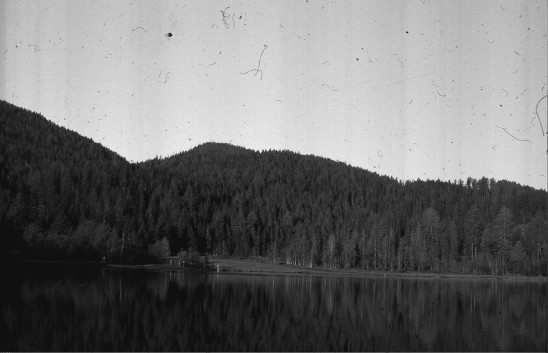
\includegraphics[width=0.5\textwidth]{images/jpg/imgproc_calib_1.jpg} }}
  \subfloat[calibration image]{{
\includegraphics[width=0.5\textwidth]{images/jpg/imgproc_calib_2.jpg} }}
  
  \subfloat[division $a / b$]{{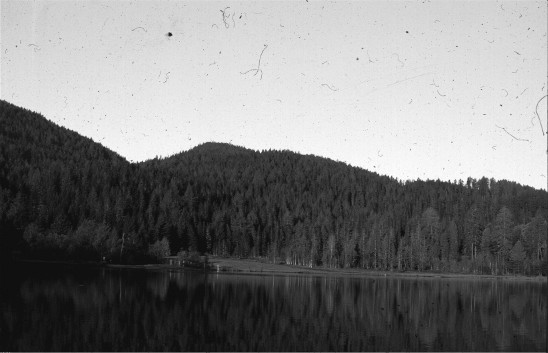
\includegraphics[width=0.5\textwidth]{images/jpg/imgproc_calib_3.jpg} }}
\end{figure}

\subsection{Point operations}

Point operations are a special class of image processing operations where the output value
at any pixel only depends on the input value at that pixel (so the operation
can be described as a function from the channel levels to the channel levels) \cite{pointwise_gimp}.
For all described operations, if the output value lies outside $[0, 1]$,
it is clipped to the respective limit.

\subsubsection{Brightness}

Adjusting brightness means adding an absolute number to each pixel value.
To increase the brightness by $k$, a function $f(b) = b + k$ is used.

\subsubsection{Contrast}

Changing contrast means compressing the brightness function so that its climb
is steeper at the middle.
To increase the contrast by a factor $k > 0$, a function $f(b) = (b - 0.5) * k + 0.5$ is used.
The brightness function gets centered around zero, steepened by factor k, then moved
back.

\subsubsection{Gamma}

Changing gamma means bending the brightness function so more of its climb
is in the dark / light area.
To apply gamma correction for a $k > 0$, a function $f(b) = b^k$ is used.
If $k < 1$, the function will be bent to the right so the majority of the climb
happens in darker areas.
If $k > 1$, the function will be bent to the right so the majority of the climb
happens in darker areas.

Different image recording (film, digital sensors) and image display (screen, print)
technologies have a different inherent gamma function (their input-output response curve)
and gamma correction is necessary to make images look good on different media.

\subsubsection{Levels}

A level operation stretches a certain section of the brightness range to
the full brightness range. Typical sensor output only has a small range of values
(this allows it to record images of various sources without risking clipping),
so it has to be stretched to look appealing.

It can be represented by $f(b) = \frac{b - k_1}{k_2 - k_1}$ where $k_1$ is the lower
and $k_2$ the upper limit of the input values.

Level stretching is also used to correct color balance. Improper color balance may
be caused by different light sources (white balance) or by sensor or film sensitivity
differences on different channels.

A simple, automatic method to adjust levels for all channels is to analyze the range
most pixel values are contained in for that channel, using that as level bounds.
This gives good results for scans of color negative film.

\subsubsection{Negative film}

For negative film, the brightness of the image gets lower as the brightness of the
source increases. To make a scan of negative film look normal it needs to be inverted:
$f(b) = 1 - b$.

Color negative film also has an orange mask (base color) that was introduced to improve
the spectral response of the dyes. This can be easily removed with appropriate
level operations:


\newsavebox\mysavebox
\begin{figure}[H]
  \centering
  \caption{Color-correcting negative scan}
  
  \subfloat[raw scan]{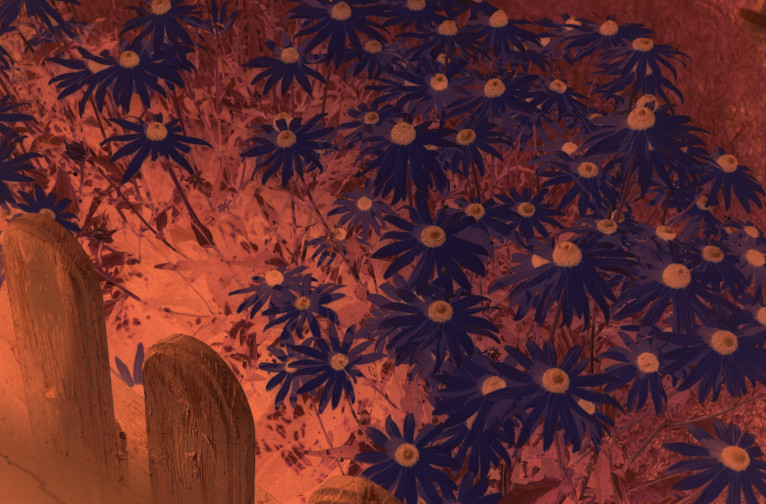
\includegraphics[width=0.49\textwidth]{images/jpg/imgproc_levels_1.jpg}} \ 
  \subfloat[inverted]{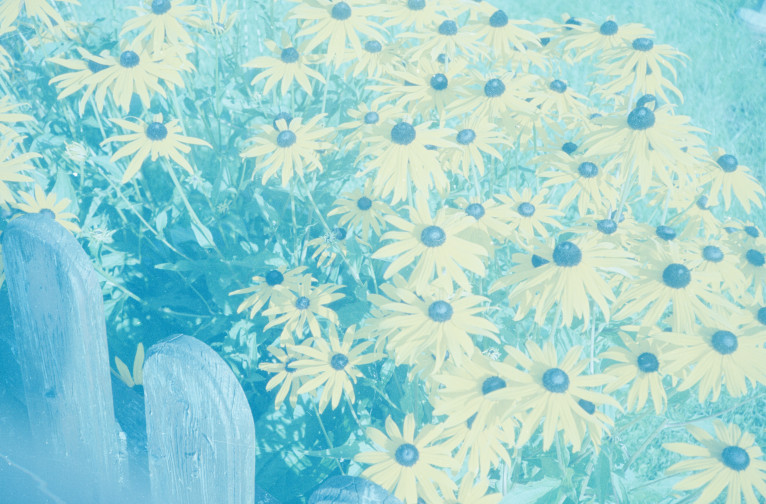
\includegraphics[width=0.49\textwidth]{images/jpg/imgproc_levels_2.jpg}}

  \subfloat[histogram of (b)]{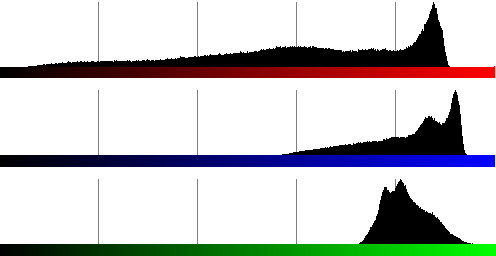
\includegraphics[width=0.49\textwidth]{images/jpg/imgproc_levels_2h.jpg}} \ 
  \subfloat[levels stretched to actual value range]{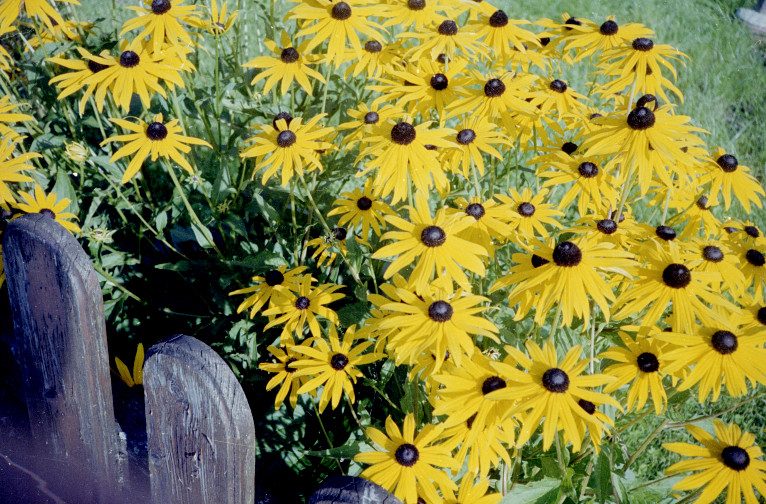
\includegraphics[width=0.49\textwidth]{images/jpg/imgproc_levels_3.jpg}}
\end{figure}

\subsection{Infrared dust / scratch removal}
\label{ssec:imgproc_dice}

Dust and scratches are an undesired but hardly avoidable artifact on scanned film material. Depending
on the condition the film is in, dust particles can be very noticeable on the scans
especially in areas of uniform color like the sky.

To deal with this, a technique often called Digital ICE \cite{inpainting_dice} was developed. It involves
scanning the film in the infrared spectrum in addition to the red, green, blue bands.
As the dyes in color film are mostly transparent to infrared, the infrared image
only shows the dust and scratches against a uniformly colored background.
From the IR image, a binary mask set at these pixels affected by dust / scratches
is created. This mask is used together with an inpainting algorithm to interpolate
the pixels affected by dust.

\begin{figure}[H]
  \centering
  \caption{Crop of slide film scan affected by dust}
  
  \subfloat[RGB image]{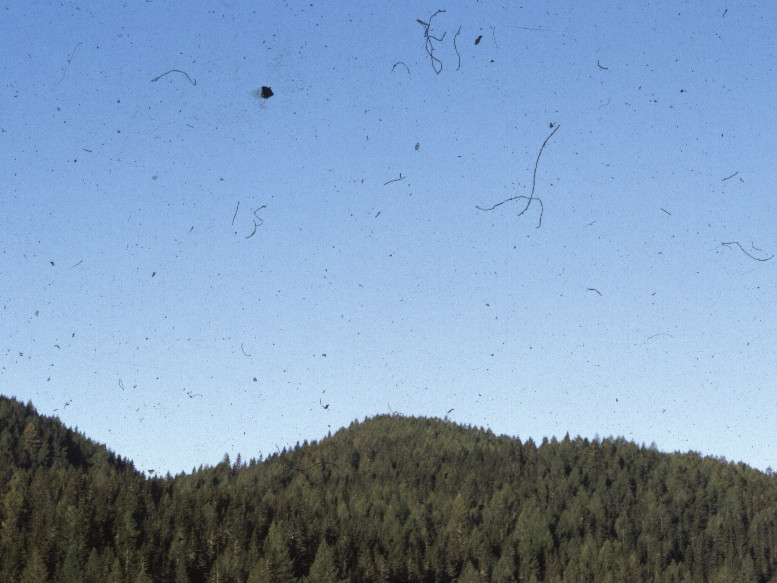
\includegraphics[width=0.49\textwidth]{images/jpg/imgproc_inpaint_1.jpg}} \ 
  \subfloat[infrared channel]{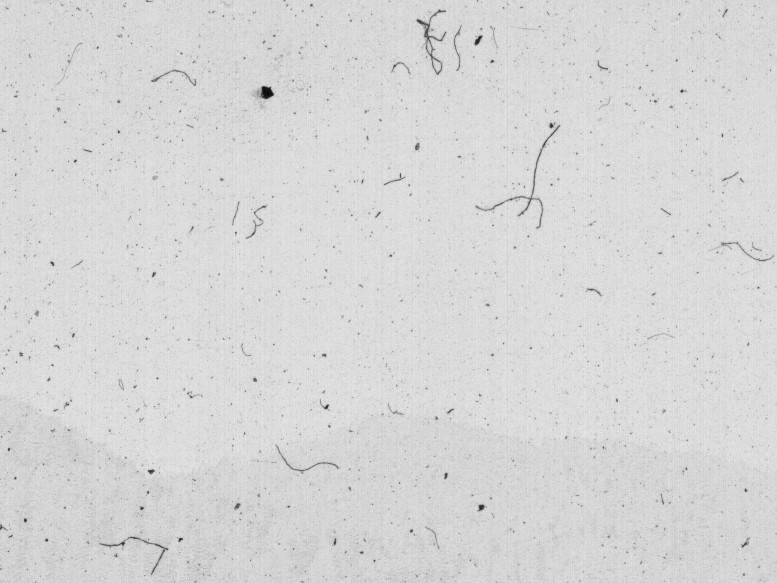
\includegraphics[width=0.49\textwidth]{images/jpg/imgproc_inpaint_2.jpg}}
\end{figure}

\subsubsection{Creating a mask}

The simple way of finding which pixels are affected by dust is apply a binary
threshold: pixels below a certain infrared brightness are considered
dust. The threshold value could be static or dynamic (adjusting so that for example 10\% of
the image is masked). Dynamic thresholds can adjust to different scanner settings /
film types, but they may under/overreact on images with unusually large / small amounts
of dust.

Finding scratches is not so easy as they don't have a strong brightness difference
from the unaffected pixels. To find them, an edge detector such as Difference-of-Gaussians
plus thresholding could be utilized.

It may also be desirable to use dilation to grow the areas of affected pixels somewhat
so the pixels just outside the mask are certainly unaffected and not harming the inpainting process.

\begin{figure}[H]
  \caption{Mask on top on image (in red) showing which pixels are affected by dust}
  \centering
  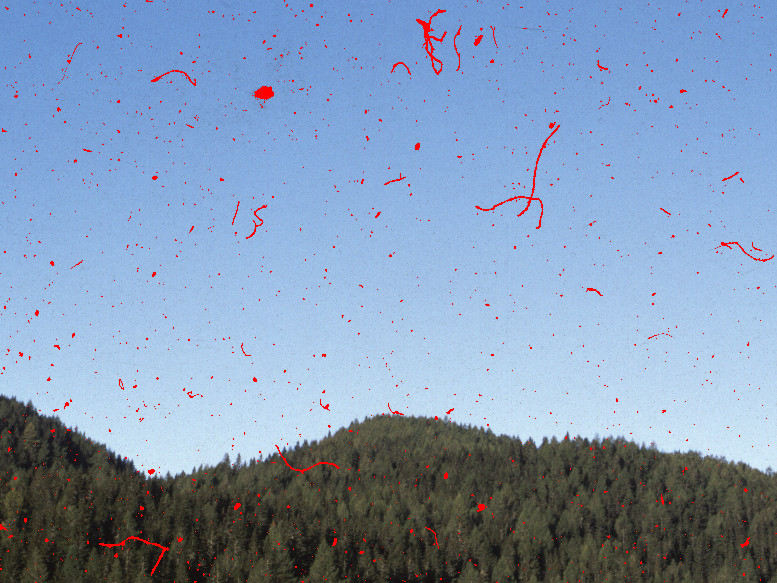
\includegraphics[width=0.5\textwidth]{images/jpg/imgproc_inpaint_3.jpg}
\end{figure}

\subsubsection{Inpainting}

Inpainting refers to the procedure of filling in certain masked, unknown
pixel values in an image using the remaining, known pixels such that the
result appears as natural as possible. Manual inpainting was a useful skill long before
the advent of digital imaging to restore old paintings / photographs or
to manipulate images by for example removing a person from it. Automatic inpainting
is an active research area in image processing and there is no single algorithm
that can claim to be the best in all scenarios. \cite{inpainting_survey}

The possibly simplest inpainting algorithm that gives decent results is called
diffusion \cite{inpainting_diffusion}. Its idea is to let image information flow from the edges of the mask
into the inpainted area until an equilibrium is reached. The steps performed are
typically:

\begin{enumerate}
  \item Blur a copy of the image by convolving it with a 3x3 kernel. Some mention
        a special choice of kernel is critical, but a simple
        $K = \begin{pmatrix} \frac{1}{9} & \frac{1}{9} & \frac{1}{9} \\
                            \frac{1}{9} & \frac{1}{9} & \frac{1}{9} \\
                            \frac{1}{9} & \frac{1}{9} & \frac{1}{9} \\ \end{pmatrix}$
        seems to provide as good results as any other.
  
  \item Combine the unblurred and blurred images by taking from the blurred image
  on the inpainted region, taking from the original image outside the inpainted region.
  
  \item Repeat steps 1-2 for as many iterations as necessary until there is no
        significant change. This depends on the diameter of the areas to be inpainted.
        For typical dust / scratch inpainting at full resolution of the scanner,
        this takes around 1000 iterations.
\end{enumerate}

The diffusion algorithm is easy to implement, fast, and predictable in its behavior.
It is however limited in that inpainted areas don't carry texture from the image
and appear somewhat blurred. This makes it unsuitable for removal of larger objects.
More advanced inpainting algorithms consider the neighborhood of the pixel to be inpainted
and search for pixels with similar neighborhood in the image, allowing texture to be propagated.
Since dust particles typically cover only small, stripe-like areas diffusion does provide
very acceptable results.

\begin{figure}[H]
  \caption{Diffusion inpainting}
  \centering
  \subfloat[1 iteration]{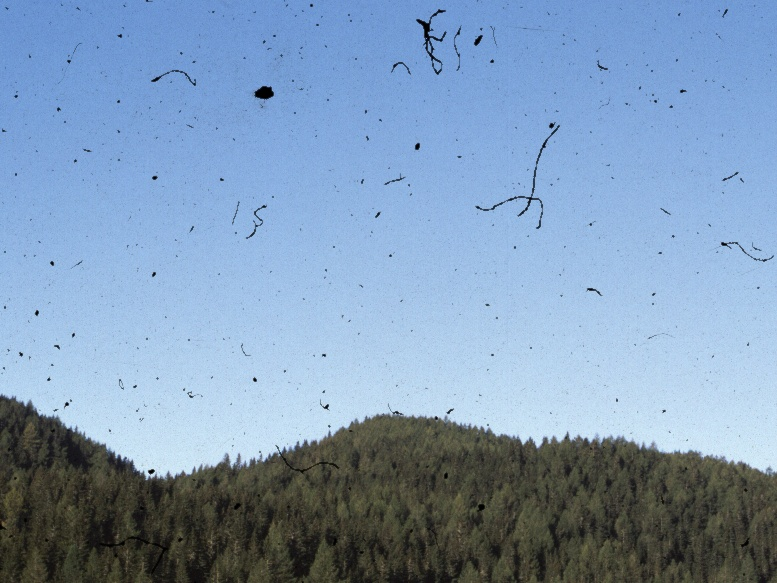
\includegraphics[width=0.49\textwidth]{images/jpg/imgproc_inpaint_4a.jpg}} \ 
  \subfloat[10 iterations]{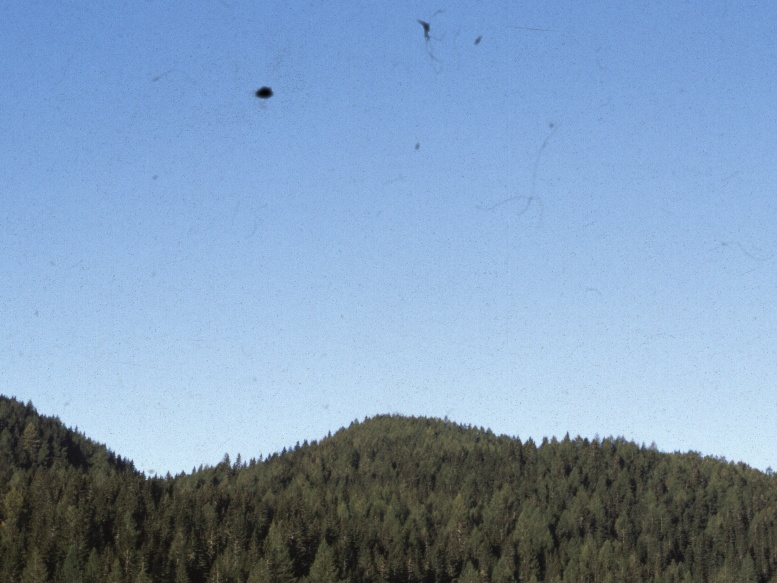
\includegraphics[width=0.49\textwidth]{images/jpg/imgproc_inpaint_4b.jpg}}
  
  \subfloat[100 iterations]{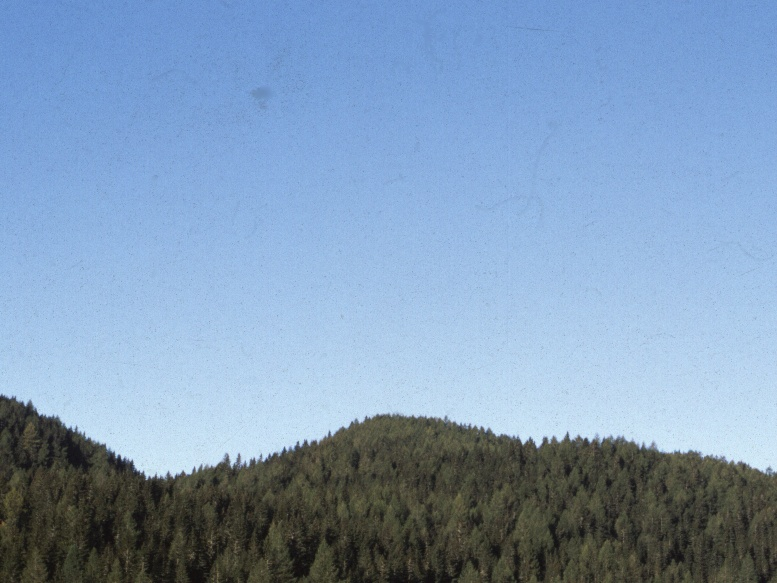
\includegraphics[width=0.49\textwidth]{images/jpg/imgproc_inpaint_4c.jpg}}
\end{figure}

\subsection{Automatic cropping}
\label{ssec:imgproc_crop}

Since the actual image on the film strip is only part of what the scanner sees,
one wants to limit the scan area so it does not include anything except the image,
but includes as much of the image as possible. An alternative is to scan the full area
and crop the resulting image afterwards. This has the advantage that it can be
automated in a program that operates on, say, each scan of one frame of a film strip.

\subsubsection{Algorithm}

As a proof-of-concept for automated cropping, a Python / OpenCV \cite{opencv}
script was created. These steps are performed to get from the raw RGB scan
to the coordinates of the crop rectangle:

\begin{enumerate}
\item {\bf Grayscale conversion}

This reduces the image from three to one channel
to simplify operations. It can be done by simply averaging the red, green, blue values at
each pixel.

\item {\bf Thresholding}

The grayscale image is converted into a binary image
by making each pixel below a specified threshold black, above white. The threshold
should be around the brightness of the unexposed sections of the film, so that these
are white and the exposed image a black rectangle (for negative film). This value
has to be adjusted based on the type of film being scanned, but can be kept constant
for all images on the same film.

\item {\bf Edge detection}

For the line detection step, we want only the border
pixels between light and dark areas to be white. This is done by applying a
Laplace operator \cite{opencv_gradient} to the threshold image.

\item {\bf Line detection (Hough transform)}

To identify lines of the image border
in the edge image, a linear Hough transform \cite{houghtransform} is used. Lines are described
in a form with two parameters $\rho, \theta$. The line is the points $(x, y)$
fulfilling the equation $\rho = x \cos \theta + y \sin \theta$. $\rho$ is the
perpendicular distance from the origin to the line and $\theta$ the angle
between the $x$ axis and a line perpendicular to the line. This has the
advantage that $\theta$ stays in the range $[0, \pi]$ for any line (for lines passing
above the origin, a negative $\rho$ is used).

A 2D accumulator matrix for all possible values of $\rho, \theta$ in this image with some
granularity is created. For each white pixel in the image and each value of $\theta$ in the
matrix, $\rho$ is computed so that the line $\rho, \theta$ goes through that pixel.
For each $\rho, \theta$ pair of a line going through the pixel, its cell in the matrix
is incremented. After having processed all pixels, the cells with values above some
threshold are parameters of lines found in the image.

\item {\bf Separate horizontal / vertical lines}

For computing intersection points between lines, it is necessary to separate
horizontal from vertical lines because lines that are almost parallel have
undesired intersection points. Lines with a $\theta$ around 0 or around $\pi$
are vertical, those with a $\theta$ around $\frac{\pi}{2}$ are horizontal.

\item {\bf Intersect lines}

Each horizontal line is intersected with each vertical line.
The intersection point $(x, y)$ for two lines in $\rho_1, \theta_1, \rho_2, \theta_2$
can be computed by solving the linear system
$\begin{pmatrix} \cos \theta_1 \sin \theta_1 \\ \cos \theta_2 \sin \theta_2 \end{pmatrix}
\begin{pmatrix} x \\ y \end{pmatrix} = \begin{pmatrix} \rho_1 \\ \rho_2 \end{pmatrix}$.

\item {\bf Classify intersections into corners}

Intersections are divided into the 4 corners by splitting the image in half
horizontally and vertically. Intersections that are not close to any corner are discarded.
One dummy point per corner (at the very corner) is inserted to make the algorithm
work even if not all corners of the frame are visible.
For each corner, the point with the greatest distance to the corner is selected
to make sure the crop frame is inside the image frame.

\item {\bf Crop rectangle}

The $x$ limits of the crop frame are from the maximum $x$ of the top left and bottom left
corner point to the minimum $x$ of the top right and bottom right corner point.
The $y$ limits of the crop frame are from the maximum $y$ of the top left and top right
corner point to the minimum $y$ of the bottom left and bottom right corner point.
This accounts for the crop points not being a straight rectangle for example because
the image is slightly rotated.

\end{enumerate}

\begin{figure}[H]
  \caption{Applying crop algorithm to image}
  \centering
  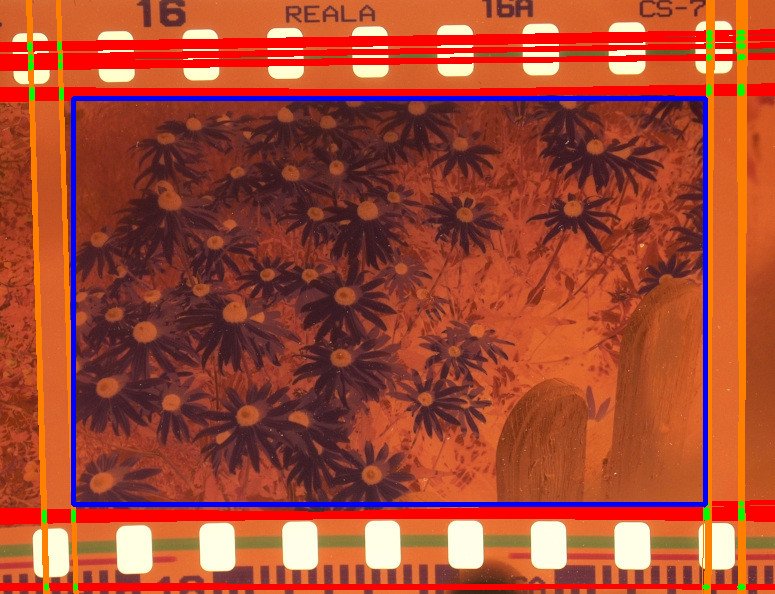
\includegraphics[width=\textwidth]{images/jpg/imgproc_autocrop_2.jpg}
\end{figure}

\subsubsection{Performance}

This algorithm uses rather basic image processing operations, but given
the correct parameters (threshold, hough granularity / sensitivity) seems to
work reliably on images with strong exposure where there is a significant brightness
difference along the entire border of the frame, which seems to include the
majority of daylight photos. For an image that however has little to no exposure
and therefore no strong brightness change on some side, thresholding will not give
a good edge and the line will not be found. Also, when scanning slide film in plastic
frames, the scanner does not pick up a significant brightness change between
the frame and dark sections of the image (it has problems differentiating high density
values). To properly crop these images as well, a more advanced procedure possibly
utilizing machine learning techniques could be used. When only a few images are
cropped incorrectly however, one can manually review all images after applying the
algorithm and still enjoy significant time savings compared to cropping every image manually.

\section{Summary}

To make the CrystalScan 7200 usable under Linux, the reverse engineering technique
of USB sniffing was employed. For this, the USB standard was summarized with particular
focus on the types and structure of control transfers \autoref{sec:usb}. After that, various methods of
sniffing USB traffic were compared \autoref{ssec:snifferscompared}. Software sniffing is done using the usbmon
Linux kernel module. To allow access to all of the payload of large packets / control transfers,
a simple patch had to be applied to this kernel module \autoref{ssec:kernelpatch}. Wireshark / tshark was used
to decode raw packets and extract control transfer parameters \autoref{ssec:wireshark}. The vendor-supplied
software was run on Windows inside VirtualBox (using the USB passthrough feature)
while letting Wireshark sniff on the Linux host \autoref{ssec:virtualbox}.

As a partial goal, the image was reconstructed from the captured packet stream \autoref{sssec:channelcombine}.
Then, the packet sequence was studied for patterns. All traffic could me modeled
using four types of transaction \autoref{ssec:transactionpatterns}. By trial and error the meaning of some of the bytes
in the transaction parameters was uncovered \autoref{appendix_meaning}. Keeping the importance of proper timing
in mind, (slightly modified versions of) the packet stream could be replayed to the device
to make a usable scanning software.

The SANE Linux scanning framework's driver only needed minimal modifications
to make it work with the scanner, most features are supported \autoref{sec:sane}.
This driver was studied to extend the description
of the transaction parameters in the previous section.

Finally, there is a lot of digital image processing required before a raw image
from the scanner becomes usable \autoref{sec:imgproc}. The basic steps include assembling the image
from the data packets, performing shading calibration, gamma and level correction.
To eliminate dust and scratches,a simple yet sufficient inpainting algorithm
was presented \autoref{ssec:imgproc_dice}. A method for automatically cropping
away the unexposed area of the film was demonstrated \autoref{ssec:imgproc_crop}.

There are some aspects of scanner behavior that make using the device
more complex and were not covered in this work:

\begin{itemize}
\item There are various patterns in which the color channel lines can be interleaved,
not just the described RGBI order. The order is chosen based on the "color format" parameter
(see \autoref{table:param15}) and possibly the resolution and color mode.

\item
The scanner has a maximum advertised resolution of 7200 dpi. The maximum line width
however is 5341 pixels, giving a horizontal resolution of only
$\frac{5341 \text{px} \cdot 25.4 \text{mm per inch}}{36 \text{mm scan area}} \approx 3768$
dpi. The 7200 dpi are only achieved in vertical direction: In a scanner,
vertical resolution can easily be increased by letting the scan head run slower, but
the maximum horizontal resolution is limited by the amount of pixels in the line sensor.
This means the resulting image has twice as many lines of the same width (compared to a 3600 dpi scan).
The image should be downscaled vertically by 50 percent to fix the stretching. The differences
in actual image detail at the two resolutions are small.

\item
After idling for about 10 minutes, the background lamp of the scanner switches off and the
device is sent into standby mode. Before sending scan commands as usual, it needs to be
woken up with a special control transfer sequence.
\end{itemize}

There are other methods of reverse engineering that could be applied to this device:
The scanner could be disassembled to analyze chips / components. Device firmware could
possibly be extracted and studied. Also the vendor supplied software / drivers (CyberView X5)
could be a target of reverse engineering. Each of these methods could give deeper insight
into the device not possible with USB sniffing. However, the simple idea of replaying
(perhaps slightly modified) versions of the captured packet stream to the device
allowed development of a working basic driver with minimal effort.

\appendix
\section*{Appendices}
\addcontentsline{toc}{section}{Appendices}
\renewcommand{\thesubsection}{\Alph{subsection}}


\subsection{Meaning of bytes in control transfer}
\label{appendix_meaning}

\subsubsection{Basic transaction}
\label{appendix_basic}

\begin{table}[H]
  \caption{Observed values for the "Main parameters" bytestring}
  \centering
  \begin{tabularx}{\textwidth}{l | X}
    Value (hex) & Description \\ \hline
    {\tt 000000000000} & Used to wait for device readiness at various points while preparing to scan. The transaction is repeated
                         until the device readiness query returns the right response.
                         \\
    {\tt 1b0000000100} & The actual "start scan" command. Is issued after transmitting all scan parameters
                         before receiving the image data. After receiving this command, the scanner
                         starts to make noise and eventually moves the scan head. \\
  \end{tabularx}
\end{table}

\subsubsection{Extra parameter transaction}
\label{appendix_extra}

\begin{table}[H]
  \caption{Observed values for the "Main parameters" bytestring}
  \centering
  \begin{tabularx}{\textwidth}{l | X}
    Value (hex) & Description \\ \hline
    {\tt 0a0000000600} & Unclear purpose \\
    {\tt 0a0000000800} & Unclear purpose \\
    {\tt 0a0000000e00} & Scan area \\
    {\tt 150000001000} & Resolution, color mode \\
    {\tt dc0000001d00} & Exposure / gain \\
  \end{tabularx}
\end{table}

Only bytes at offset 0 and 4 are set. The byte at offset 0 identifies the
purpose of this transaction (e.g. set resolution, scan area). The byte value at offset 4 equals
the number of bytes that are later transferred in the "Extra parameter"
stage.

Sometimes, the same byte 0 (purpose) is used with varying bytes 4 (length).
It is unclear whether such extra parameter bytestrings of different lengths
are related to each other. Usually, only one of these lengths is used to transmit
a string that actually carries relevant information (i.e. it changes when
changing settings in the vendor software).

For three main parameter strings, the extra parameter string varies
with different scan settings. The meaning of some bytes in these strings
can be discovered by varying one setting and observing the change in the
string. Most of the information presented here, however,
is taken from comments in the code of the SANE backend for this device.
For each of the three parameters, an example string from an actual
scan is analyzed:

\paragraph{0a0000000e00}

This parameter string is used to set the boundaries of the scan
frame / scan area. The corresponding extra parameter bytestring
consists of 5 2-byte little-endian values:

\begin{table}[H]
  \caption{Decoding extra parameters for "0a0000000e00"}
  \centering
  \begin{tabularx}{\textwidth}{p{1cm} | p{1cm} | X}
    Offset & Value (hex) & Description \\ \hline
    0-1 & {\tt 1200} & Constant representing "scan frame" \\
    2-3 & {\tt 0a00} & Size of rest of frame (10 bytes), constant \\
    4-5 & {\tt 8000} & Index of frame, constant \\
    6-7 & {\tt 6f02} & X coordinate of top left corner of area (units unknown) \\
    8-9 & {\tt 0f00} & Y coordinate of top left corner of area (units unknown) \\
    10-11 & {\tt 2829} & X coordinate of bottom right corner of area (units unknown) \\
    12-13 & {\tt f819} & Y coordinate of bottom right corner of area (units unknown) \\
  \end{tabularx}
  
  \vspace{5mm}
  Information taken from comments in this C code: \cite[\texttt{pieusb\_scancmd.c}]{sane_code}
  \label{table:param0a}
\end{table}

The ratio of x distance to y distance in this example is:

$\frac{\textrm{0x2928} - \textrm{0x026f}}{\textrm{0x19f8} - \textrm{0x000f}} = \frac{9913}{6633} \approx 1.494$.

This matches the proportions of a 35mm film frame: $\frac{36 \textrm{mm}}{24 \textrm{mm}} = 1.5$.

\paragraph{150000001000} This is used to set many different scan parameters
such as resolution, color mode, color depth etc. Multi-byte
values are in little-endian format.

\begin{table}[H]
  \caption{Decoding extra parameters for "150000001000"}
  \centering
  \begin{tabularx}{\textwidth}{p{1cm} | p{1cm} | X}
    Offset & Value (hex) & Description \\ \hline
    0-1 & {\tt 000f} & Constant representing "scan parameters" \\
    2-3 & {\tt b004} & Scan resolution (in dots per inch) \\
    4 & {\tt 80} & Color mode ({\tt 80} - RGB, {\tt 90} - RGB + infrared) \\
    5 & {\tt 80} & Color depth ({\tt 04} - 8 bit, {\tt 20} - 16 bit) \\
    6 & {\tt 04} & Color format \\
    7 & {\tt 00} & unused \\
    8 & {\tt 01} & Byte order of pixel value ({\tt 01} - little endian) \\
    9 & {\tt 00} & Bitmap for various quality settings ({\tt 80} - fast infrared,
                                                        {\tt 08} - skip calibration,
                                                        {\tt 02} - sharpen) \\
    10-11 & {\tt 0000} & unused \\
    12 & {\tt 01} & halftone pattern \\
    13 & {\tt 80} & line threshold \\
    14-15 & {\tt 1000} & unknown \\
  \end{tabularx}
  
  \vspace{5mm}
  Information taken from comments in this C code: \cite[\texttt{pieusb\_scancmd.c}]{sane_code}
  \label{table:param15}
\end{table}

\paragraph{dc0000001d00} This is used to set some parameters such as exposure time
per channel and digitizer gain / offset. Multi-byte
values are in little-endian format.

\begin{table}[H]
  \caption{Decoding extra parameters for "dc0000001d00"}
  \centering
  \begin{tabularx}{\textwidth}{p{1cm} | p{2.5cm} | X}
    Offset & Value (hex) & Description \\ \hline
    0-5 & {\tt 7e26661c1515} & exposure time for red, green, blue channel
                               (one 16-bit little-endian value per channel) \\
    6-8 & {\tt 171411} & Digitizer offset for red, green, blue channel
                               (one 8-bit value per channel) \\
    9-11 & {\tt 000000} & unused \\
    12-14 & {\tt 212121} & Digitizer gain for red, green, blue channel
                               (one 8-bit value per channel) \\
    15 & {\tt 07} & light \\
    16 & {\tt 00} & extra entries \\
    17 & {\tt 00} & double times \\
    18-19 & {\tt 790b} & Exposure time for infrared channel \\
    20-21 & {\tt 1400} & Digitizer offset for infrared channel \\
    22 & {\tt 0f} & Digitizer gain for infrared channel \\
    23-28 & {\tt 000000000000} & unused \\
  \end{tabularx}
  
  \vspace{5mm}
  Information taken from comments in this C code: \cite[\texttt{pieusb\_scancmd.c}]{sane_code}
  \label{table:paramdc}
\end{table}

\subsubsection{Status transaction}
\label{appendix_status}
\begin{table}[H]
  \caption{Observed values for the "Main parameters" bytestring}
  \centering
  \begin{tabularx}{\textwidth}{l | X}
    Value (hex) & Description \\ \hline
    {\tt 030000000e00} & Unknown purpose \\
    {\tt 080000008000} & Unknown purpose \\
    {\tt 0f0000001200} & Main image parameters \\
    {\tt 18000014dc00} & Mask specifying which pixels of the sensor contribute to the
                         output data (useful for calibration) \\
    {\tt d70000006700} & Gain / offset values \\
    {\tt dd0000001200} & Basic scanner status. Sent in regular intervals by the
                                               vendor software while the scanner is idle. \\

  \end{tabularx}
  \label{table:read_param}
\end{table}

Many different main parameter combinations are used for status reads. As most of the returned
information is not critical for basic scanning functionality, not all bytestrings are
studied in detail.

Bytes at offset 0, 3, 4 can be set. Bytes 3 and 4 specify the number of bytes to
be read from the bulk endpoint: $256 * b_3 + b_4$.

\paragraph{0f0000001200}

This parameter string is used to receive information about the image produced by the scanner.
It contains the image width / height, this is needed to use the proper image transaction
parameters. Multi-byte values are in little-endian format.

\begin{table}[H]
  \caption{Decoding status response for "0f0000001200"}
  \centering
  \begin{tabularx}{\textwidth}{p{1cm} | p{2cm} | X}
    Offset & Value (hex) & Description \\ \hline
    0-1 & {\tt 7406} & Line width (pixels) \\
    2-3 & {\tt 2c04} & Number of lines in the image \\
    4-5 & {\tt e80c} & Number of bytes in the image \\
    6 & {\tt 08} & Filter offset 1 \\
    7 & {\tt 08} & Filter offset 2 \\
    8-11 & {\tt 00000000} & Exposure period \\
    12-13 & {\tt 7266} & SCSI transfer rate \\
    14-15 & {\tt 0000} & Number of lines in buffer right now \\
    16-17 & {\tt 0000} & unused \\
  \end{tabularx}
  
  \vspace{5mm}
  Information taken from comments in this C code: \cite[\texttt{pieusb\_scancmd.c}]{sane_code}
  \label{table:imageparam_query}
\end{table}


\subsection{USB traffic during an example scan}
\label{appendix_actualscan}

\begin{table}[H]
  \caption{Scan parameters}
  \centering
  \begin{tabularx}{\textwidth}{p{3cm} | X}
    Setting & Value \\ \hline
    Scan mode & Pre-scan \\
    Resolution & 300 dpi (main image), 3600 dpi (calibration image) \\
    Color mode & RGB (main image), RGBI (calibration image) \\
    Color depth & 1 byte per pixel (main image), 2 bytes per pixel (calibration image) \\
    \end{tabularx}
\end{table}

\begin{tabularx}{\textwidth}{p{0.2cm}|p{2.3cm}|p{2cm}|X}
  \caption{Transactions of the scan} \\
  Ty\-pe & Main parameters (hex) & Extra parameters (hex) & Description \\ \hline
  \endfirsthead
  \caption{Transactions of the scan (continued)} \\
  Ty\-pe & Main parameters (hex) & Extra parameters (hex) & Description \\ \hline
  \endhead
  \\ \caption*{Transaction types: B - Basic, E - Extra parameter, S - Status, I - Image} \\
  \endfoot
  \\ \caption*{Transaction types: B - Basic, E - Extra parameter, S - Status, I - Image} \\
  \endlastfoot
  S & {\tt dd0000001200} &  & Idle status query \autoref{appendix_status} \\
  B & {\tt 000000000000} &  & Readiness check \autoref{ssec:basic_trans} \\
  E & {\tt 0a0000000800} & \tt 1300040002 006400 & \\
  E & {\tt 0a0000000800} & \tt 1300040004 006400 & \\
  E & {\tt 0a0000000800} & \tt 1300040008 006400 & \\
  E & {\tt 0a0000000800} & \tt 1400040002 006400 & \\
  E & {\tt 0a0000000800} & \tt 1400040004 006400 & \\
  E & {\tt 0a0000000800} & \tt 1400040008 006400 & \\
  E & {\tt 0a0000000600} & \tt 9500000000 00 & \\
  S & {\tt 080000008000} &  & \\
  E & {\tt 0a0000000e00} & \tt 12000a0080 0000000000 b829e71a & Set scan area \autoref{table:param0a} \\
  E & {\tt 0a0000000600} & \tt 1700020001 00 & \\
  S & {\tt 030000000e00} &  & \\
  B & {\tt 000000000000} &  & Readiness check \autoref{ssec:basic_trans} \\
  S & {\tt d70000006700} &  & Read gain / offset values \autoref{appendix_status} \\
  E & {\tt dc0000001d00} & \tt 0000000000 0000000000 0000000000 07001a790b 00fe0f0000 00000000
                         & Set exposure settings \autoref{table:paramdc} \\
  B & {\tt 000000000000} &  & Readiness check \autoref{ssec:basic_trans} \\
  E & {\tt 150000001000} & \tt 000f2c0180 0404000100 0000008010 00 & \autoref{table:paramdc} \\
  B & {\tt 1b0000000100} &  & Start scan \autoref{ssec:basic_trans} \\
  B & {\tt 000000000000} &  & Readiness check \autoref{ssec:basic_trans}, 3rd attempt is successful \\ 
  S & {\tt d70000006700} &  & Read gain / offset values \autoref{appendix_status} \\
  E & {\tt dc0000001d00} & \tt 7b1e2f168c 1017141000 0000212121 070000790b 14000f0000 00000000
                         & Set exposure settings \autoref{table:paramdc} \\
  I & {\tt 080000000400} &  & Transfer 4 lines / 42728 bytes of the calibration image \autoref{ssec:rcv_calibimage} \\
  B & {\tt 000000000000} &  & Readiness check \autoref{ssec:basic_trans}, 2nd attempt is successful \\
  I & {\tt 08000000ac00} &  & Transfer 172 lines / 1837304 bytes of the calibration image \autoref{ssec:rcv_calibimage}  \\
  S & {\tt d70000006700} &  & Read gain / offset values \autoref{appendix_status} \\
  E & {\tt dc0000001d00} & \tt 7b1e2f168c 1017141000 0000212121 070000790b 14000f0000 00000000
                         & Set exposure settings \autoref{table:paramdc} \\
  I & {\tt 080000000400} &  & Transfer 4 lines / 42728 bytes of the calibration image \autoref{ssec:rcv_calibimage} \\
  B & {\tt 000000000000} &  & Readiness check \autoref{ssec:basic_trans}, 2nd attempt is successful \\
  S & {\tt 18000014dc00} &  & Read row mask \autoref{appendix_status} \\
  S & {\tt 0f0000001200} &  & Get size of the main image \autoref{table:imageparam_query}.
                              Returned status is {\tt bc011f01bc01}... This means the
                              image has 287 * 3 (color channels) = 861 lines of 444 bytes each. \\
  B & {\tt 000000000000} &  & Readiness check \autoref{ssec:basic_trans}, 3rd attempt is successful \\
  I & {\tt 08000000d800} &  & Transfer 216 lines / 95904 bytes of the main image \autoref{ssec:rcv_mainimage}.
                              Repeated 3 times.
                              In this case, they are transferred in chunks of 216 lines. It would also
                              be fine to use the simpler scheme with 255 lines / transaction. \\
  I & {\tt 08000000d500} &  & Transfer the rest, that is 213 lines / 94572 bytes of the main image. \\
\end{tabularx}

\newcounter{firstbib}
\pagebreak

\renewcommand{\refname}{References}
\begin{thebibliography}{}

  \item[]\hspace{-\labelwidth}\hspace{-\labelsep}\textbf{USB standard}

  \bibitem{uc} USB Complete: Everything You Need to Develop
               Custom USB Peripherals (\nth{3} edition).
               Jan Axelson, Lakeview Research LLC 2012.
               ISBN: {\tt   978-1-931448-03-1}
               
  \item[]\hspace{-\labelwidth}\hspace{-\labelsep}\textbf{USB sniffing}
  
  \bibitem{usbmon} The usbmon: USB monitoring framework. Pete Zaitcev,
  Proceedings of the Linux Symposium, Volume Two, July 20-23 2005.
  
  \item[]\hspace{-\labelwidth}\hspace{-\labelsep}\textbf{Image processing}
  
  \bibitem{inpainting_survey} A survey of inpainting algorithms. Marcelo Bertalmıo, Vicent Caselles, Simon Masnou,
  Guillermo Sapiro:
  \url{http://math.univ-lyon1.fr/homes-www/masnou/fichiers/publications/survey.pdf}
  
  \bibitem{inpainting_diffusion} Fast Digital Image Inpainting: Manuel M. Oliveira,
  Brian Bowen, Richard McKenna, Yu-Sung Chang. 
  Proceedings of the International Conference on Visualization, Imaging and Image Processing (VIIP 2001).
  
  \bibitem{houghtransform} Use of the Hough transformation to detect lines and curves in pictures.
  Richard O. Duda, Peter E. Hart, Communications of the ACM, Volume 15 Issue 1, Jan. 1972,
  pages 11-15.
  
  \setcounter{firstbib}{\value{enumiv}}
\end{thebibliography}

\renewcommand{\refname}{Links}
\begin{thebibliography}{}
  \setcounter{enumiv}{\value{firstbib}}
  \item[]\hspace{-\labelwidth}\hspace{-\labelsep}\textbf{The device}
  
  \bibitem{rcs}
  \url{https://reflecta.de/en/products/detail/~id.15/reflecta-CrystalScan-7200.html}
  
  \bibitem{rcs_review}
  \url{http://www.filmscanner.info/en/ReflectaCrystalScan7200.html}
  
  \bibitem{vuescan}
  \url{https://www.hamrick.com/}
  
  \bibitem{silverfast}
  \url{http://www.silverfast.com/scanner-software/en.html}
  
  \item[]\hspace{-\labelwidth}\hspace{-\labelsep}\textbf{USB standard}
  
  \bibitem{usbstd} Universal Serial Bus Specification, Revision 2.0.
                   April 27, 2000. Available at
                   \url{http://www.usb.org/developers/docs/usb20_docs/}

  \bibitem{usbhid}
  \url{http://www.usb.org/developers/hidpage/HID1_11.pdf} \\
  USB HID Device Class Definition. Describes the structure of HID reports.
  
  \bibitem{usbusage}
  \url{http://www.usb.org/developers/hidpage/Hut1_12v2.pdf} \\
  USB HID Usage Tables. Describes the meaning of bytes in HID reports.

  \item[]\hspace{-\labelwidth}\hspace{-\labelsep}\textbf{USB sniffing}


  \bibitem{analyzerbenefits}
  \url{https://www.totalphase.com/solutions/apps/usb-analyzer-benefits/}

  \bibitem{usbmon_others}
  \url{http://permalink.gmane.org/gmane.linux.usb.general/101338} \\
  Others describing issues with {\it} usbmon truncating payloads
  
  \bibitem{debkernel}
  \url{https://www.debian.org/releases/stretch/amd64/ch08s06.html.en}

  \bibitem{wireshark}
  \url{https://www.wireshark.org/} \\
  Homepage of the Wireshark network protocol analyzer
  
  \bibitem{wireshark_tshark}
  \url{https://www.wireshark.org/docs/man-pages/tshark.html}
  
  \bibitem{wireshark_userguide}
  \url{https://www.wireshark.org/docs/wsug_html} \\
  Wireshark User's Guide

  \bibitem{vbox}
  \url{https://www.virtualbox.org/}

  \item[]\hspace{-\labelwidth}\hspace{-\labelsep}\textbf{Vendor-supplied scanner software}
  \bibitem{cvx5}
  \url{https://reflecta.de/de/downloads/drivers2/~nm.50~nc.108/Treiber-und-Software.html}

  \item[]\hspace{-\labelwidth}\hspace{-\labelsep}\textbf{Image editing}

  \bibitem{gimp}
  \url{https://www.gimp.org/}

  \item[]\hspace{-\labelwidth}\hspace{-\labelsep}\textbf{Developing USB drivers}

  \bibitem{pyusb}
  \url{https://github.com/pyusb/pyusb} \\
  Control USB devices from Python. Has a great tutorial on using the software.
  
  \item[]\hspace{-\labelwidth}\hspace{-\labelsep}\textbf{SANE}
  
  \bibitem{saneproject}
  \url{http://www.sane-project.org/}
  
  \bibitem{sane_standard}
  \url{http://www.sane-project.org/sane.pdf} \\
  The SANE standard
  
  \bibitem{sane_develop}
  \url{http://sane-project.org/backend-writing.txt} \\
  General guidelines on writing SANE backends
  
  \bibitem{sane_develop_re}
  \url{http://www.meier-geinitz.de/sane/misc/develop.html} \\
  How to develop SANE backends without documentation (using reverse engineering)
  
  \bibitem{sane_code}
  \url{https://gitlab.com/sane-project/backends/tree/master/backend} \\
  Code repository (Git)
  
  \item[]\hspace{-\labelwidth}\hspace{-\labelsep}\textbf{Image processing}
  
  \bibitem{pointwise_gimp}
  \url{https://pippin.gimp.org/image-processing/chap_point.html}
  
  \bibitem{inpainting_dice}
  \url{http://asf.com/products/ice/FilmICESpecs/}
  
  \bibitem{opencv}
  \url{https://opencv.org/}
  
  \bibitem{opencv_gradient}
  \url{https://docs.opencv.org/3.0-beta/doc/py_tutorials/py_imgproc/py_gradients/py_gradients.html}
\end{thebibliography}



\end{document}
